% chapters/glitch.tex
%
% Copyright 2023 Alexander Lyttle.
%
% This work may be distributed and/or modified under the conditions of the
% LaTeX Project Public License (LPPL) version 1.3 or later.
%
% The latest version of this license is in
% https://www.latex-project.org/lppl.txt and version 1.3 or later is part of
% all distributions of LaTeX version 2005/12/01 or later.
%
%
\chapter[Acoustic glitches]{Acoustic glitches as a signature of helium abundance}\label{chap:glitch}

A glitch arises from a sharp structural variation in the star.

Explain that glitches can be a signature of helium abundance. If we can model the glitch consistently between models and observed stars, we can add parameters to the HBM which contain information about helium.

In this chapter, we explore the theoretical background of acoustic glitches

\section[1D example]{A one-dimensional example of a glitch}\label{sec:1d-glitch}

A rapid variation in the structure of a medium induces an oscillation (\(\delta\omega\)) in the eigenfrequencies. To demonstrate this, we will explore a simple one-dimensional example \citep[e.g][]{Verner2005}. Consider a medium bound from \(x=0\) to \(x=L\) in which pressure waves can propagate at constant speed \(c\). The longitudinal displacement of the wave \(\xi\) must obey the wave equation,
%
\begin{equation}
    \frac{\partial^2\xi(x, t)}{\partial t^2} = c^2 \frac{\partial^2\xi(x, t)}{\partial x^2},
\end{equation}
%
at a given position \(x\) and time \(t\). A general solution to the wave may be written as a sum of right- and left-travelling waves. In terms of the angular frequency \(\omega\), wave number \(k\), and complex coefficients \((A, B)\),
%
\begin{equation}
    \xi(x, t) = A \ee^{i (\omega t - k x)} + B \ee^{i (\omega t + k x)},
\end{equation}
%
where \(\omega\) and \(k\) satisfy \(\omega = c k\). Solving for the boundary condition \(\xi(0, t) = 0\) we find \(B = - A\). Substituting Euler's formula, \(A = (r/2) \ee^{i\phi}\), we can write the real solution for \(\xi\) as,
%
\begin{equation}
    \real\left[\xi(x, t)\right] = r \sin k x \sin(\omega t + \phi),
\end{equation}
%
representing the physical component of the wave, where \(r\) and \(\phi\) are the amplitude and temporal phase respectively. Solutions for \(\omega\) which satisfy \(\xi(L, t)=0\) may then be found,
%
\begin{equation}
    \omega_n = c \frac{n \pi}{L}, \label{eq:omega-n}
\end{equation}
%
where \(n\) is a non-zero integer (the \(n=0\) solution would give \(\xi=0\) everywhere).

Now, let us suppose there is a small structural perturbation (or glitch) in the medium at position \(x_0\) with half-width \(\delta x\). Figure \ref{fig:1d-diagram} shows this system divided into 3 regions, with region 2 containing the glitch. In region 2, the speed of sound is \(c + \delta c\) and the corresponding wave number is \(k + \delta k\). We want to find the frequencies which correspond to standing waves in this system and compare them to that of the homogeneous medium above. We will show that the resulting eigenfrequencies oscillate with an amplitude and period that relates to the properties of the glitch.

Firstly, we propose solutions to the wave for each region by considering reflection and transmission at each boundary. Initially ignoring the wave superposed by a reflection at \(x=L\),
%
\begin{align}
    \xi_1(x, t) &= \ee^{i(\omega t - k x)} + A \ee^{i(\omega t + k x)}, \label{eq:xi1-r} \\
    \xi_2(x, t) &= B\ee^{i(\omega t - (k + \delta k) x)} + C \ee^{i(\omega t + (k + \delta k) x)}, \label{eq:xi2-r} \\
    \xi_3(x, t) &= D \ee^{i(\omega t - k x)}, \label{eq:xi3-r}
\end{align}
%
where complex coefficients \(A\) and \(C\) represent reflections, and \(B\) and \(D\) represent transmissions, at \(x_0 \pm \delta x\) respectively. Later, we will substitute the left-travelling wave (\(- \xi\{-k, -\delta k\}\)) after determining the values of the coefficients.

\begin{figure}
    \centering
    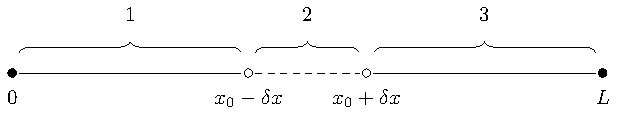
\includegraphics{figures/glitch-1d-example-diagram.pdf}
    \caption[A diagram showing a one-dimensional medium with a small structural perturbation.]{A diagram showing a one-dimensional medium split into three regions. 1: Fixed at \(x=0\) with a constant speed of sound \(c\); 2: A small structural perturbation centred at \(x=x_0\) with width \(2\delta x\) and constant speed of sound \(c + \delta c\); 3: Fixed at \(x=L\) with a constant speed of sound \(c\).}
    \label{fig:1d-diagram}
\end{figure}

The boundary conditions for this system are found by enforcing spacial continuity at \(x - \delta x\) and \(x + \delta x\),
%
\begin{align*}
    \xi_1(x_0 - \delta x, t) &= \xi_2(x_0 - \delta x, t), \\
    \xi_2(x_0 + \delta x, t) &= \xi_3(x_0 + \delta x, t), \\
    \frac{\partial \xi_1}{\partial x}(x_0 - \delta x, t) &= \frac{\partial \xi_2}{\partial x}(x_0 - \delta x, t), \\
    \frac{\partial \xi_2}{\partial x}(x_0 + \delta x, t) &= \frac{\partial \xi_3}{\partial x}(x_0 + \delta x, t).
\end{align*}
%
Solving these simultaneously with the Python package \textsc{sympy} gives the following equations for the complex coefficients\footnote{The code for these derivations are available at \url{\gitremote/tree/\gitbranch/notebooks}},
%
\begin{align}
    A &= \delta k (2k + \delta k) (1 - \ee^{4i \delta x (k + \delta k)}) \ee^{- 2i k (x_0 - \delta x)} \alpha^{-1}, \\
    B &= 2 k (2k + \delta k) \ee^{4i \delta x (k + \delta k)} \ee^{i \delta k (x_0 - \delta x)} \alpha^{-1}, \\
    C &= 2 k \delta k \ee^{- i (x_0 - \delta x) (2k + \delta k)} \alpha^{-1}, \\
    D &= 4 k (k + \delta k) \ee^{2 i \delta x (2k + \delta k)} \alpha^{-1},
\end{align}
%
where,
\begin{equation}
    \alpha = (2k + \delta k)^2 \ee^{4 i \delta x (k + \delta k)} - \delta k^2.
\end{equation}
%

Now we have solutions for the coefficients, we can superpose the right-travelling wave, \(\xi\{k, \delta k\} \rightarrow - \xi\{-k, -\delta k\}\) to get the full solution for the wave function. Substituting \(k \rightarrow -k\) and \(\delta k \rightarrow -\delta k\) into the coefficients yields their complex conjugates, \((\overline{A},\overline{B},\overline{C},\overline{D})\). This allows us to rewrite the wave functions into a more flexible form. For example, substituting Euler's formula, \(A = (r_A/2) \ee^{i\phi_A}\) and \(\overline{A} = (r_A/2) \ee^{-i\phi_A}\), Equation \ref{eq:xi1-r} now becomes,
%
\begin{equation}
    \xi_1(x, t) = \ee^{i \omega t} \left[ \frac{r_A}{2} \left( \ee^{i(kx + \phi_A)} - \ee^{-i(kx + \phi_A)} \right) - \left( \ee^{ikx} - \ee^{-ikx} \right) \right] \label{eq:xi1}
\end{equation}
%
where its real component is,
\begin{equation}
    \real\left[\xi_1(x, t)\right] = \sin \omega t \left[2 \sin kx - r_A \sin(kx + \phi_A)\right].
\end{equation}
%
However, this does not satisfy the boundary condition that the displacement is always zero at \(x=0\); \(\xi_1(0, t) = - r_A \sin \omega t \sin(\phi_A) \neq 0\). To do so, we introduce a small displacement phase \(\epsilon\) caused by the glitch, and let \(x \rightarrow x + \epsilon\). We will determine \(\epsilon\) shortly. In the meantime, superposing the right-travelling wave and substituting Euler's formula into Equations \ref{eq:xi2-r} and \ref{eq:xi3-r}, we can write the real components of the wave functions,
%
% \begin{align}
%     \xi_3(x, t) = \frac{r_A}{2} \ee^{i \omega t} \left[ \ee^{i(k(x + \epsilon) + \phi_A)} - \ee^{-i(k(x + \epsilon) + \phi_A)} \right],
% \end{align}
%
% with a real solution in trigonometric form,
%
\begin{align}
    \real[\xi_1(x, t)] &= \sin \omega t \left\{2 \sin[k (x + \epsilon)] - r_A \sin[k(x + \epsilon) - \phi_A]\right\} \label{eq:xi1-real} \\
    \real[\xi_2(x, t)] &= \sin \omega t \left\{ r_B \sin[(k + \delta k)(x + \epsilon) - \phi_B] - r_C \sin[(k + \delta k)(x + \epsilon) - \phi_C]\right\} \\
    \real[\xi_3(x, t)] &= \sin \omega t \left\{r_D \sin[k(x + \epsilon) - \phi_D]\right\} \label{eq:xi3-real}
\end{align}
%
Imposing the boundary condition \(\xi_1(0, t) = 0\), we solve Equation \ref{eq:xi1-real} for \(\epsilon\) at \(x=0\),
%
\begin{align}
    \epsilon &= \frac{1}{k} \tan^{-1}\left( \frac{(r_A / 2) \sin(\phi_A)}{1 - (r_A/2) \cos(\phi_A)} \right), \notag\\
    &= \frac{1}{k} \tan^{-1}\left( \frac{\imag[A]}{1 - \real[A]} \right). \label{eq:1d-phase}
\end{align}
%

Finally, we can impose the boundary condition \(\xi_3(L, t) = 0\) to solve for \(\omega\). Setting Equation \ref{eq:xi3-real} to zero, we can rewrite it in terms of the real and imaginary components of \(D\),
%
\begin{align}
    \sin \omega t \left\{r_D \sin[k(L + \epsilon) - \phi_D]\right\} &= 0, \quad (\div \sin \omega t) \notag \\
    r_D \cos \phi_D \sin[k(L + \epsilon)] - r_D \sin \phi_D \cos[k(L + \epsilon)] &= 0, \notag \\
    \real[D] \sin[k(L + \epsilon)] - \imag[D] \cos[k(L + \epsilon)] &=0. \label{eq:1d-glitch-sol}
\end{align}
%
The glitch affects the amplitude and phase of the wave, because if we set \(\epsilon = 0\) and \(D = 1\) we recover the homogeneous frequency solutions (Equation \ref{eq:omega-n}). Unfortunately, solving Equation \ref{eq:1d-glitch-sol} for \(\omega\) is not possible analytically. However, we can find individual roots (or modes, \(\omega_n\)) numerically.

We find \(\omega_n\) by solving Equation \ref{eq:1d-glitch-sol} using Newton's method for \(n = 1,\dots,50\), with \(c=1\), \(L=1\), and several values of \(x_0\), \(\delta x\), and \(\delta c\). Initial guesses are obtained from the homogeneous medium solutions (\(\omega_n^0\)) in Equation \ref{eq:omega-n}. The difference between the solutions for \(\omega_n\) and those from the homogeneous medium, \(\delta \omega_n = \omega_n - \omega_n^0\), are shown in Figure \ref{fig:1d-results}. We can see an oscillation in \(\delta\omega\) induced by the glitch. Physically, this arises from the change in phase required to satisfy the boundary conditions of the glitch region. As the wave nodes pass in and out of the region with changing \(n\), the sensitivity of the wave to the glitch oscillates. The overall sensitivity to the glitch depends on how much the wave changes inside the glitch, hence why low \(n\) modes have smaller \(\delta\omega\).

The functional form of \(\delta\omega\) appears to have a linear component and a short period oscillation modulated by a longer period. As the location of the glitch (\(x_0\)) gets smaller, the short-term oscillation period of \(\delta\omega\) decreases. If we imagine the spacial distribution of nodes in the system as a function of \(n\), the density of nodes is larger towards the centre of the system. The oscillation arises from the nodes passing in and out of the glitch region with changing \(n\). Therefore, where the density of wave nodes is higher, we expect the oscillation period of \(\delta\omega\) to be shorter. Similarly, as the the half-width of the glitch (\(\delta x\)) increases, the longer-term modulation period increases. 

Furthermore, an increasing change in sound speed (\(\delta c\)) increases the amplitude of \(\delta\omega\). This result is intuitive, as we expect a perturbation in \(c\) to be proportional to a perturbation in \(\omega\). Finally, increasing both \(\delta x\) and \(\delta c\) increases the slope of \(\delta\omega\). The sensitivity of a mode to the glitch increases with \(n\) and depends on how much the wave changes in the glitch region. A larger glitch allows modes of smaller \(n\) to `see' the glitch region, thus increasing the linear slope of \(\delta\omega\).

\begin{figure}
    \centering
    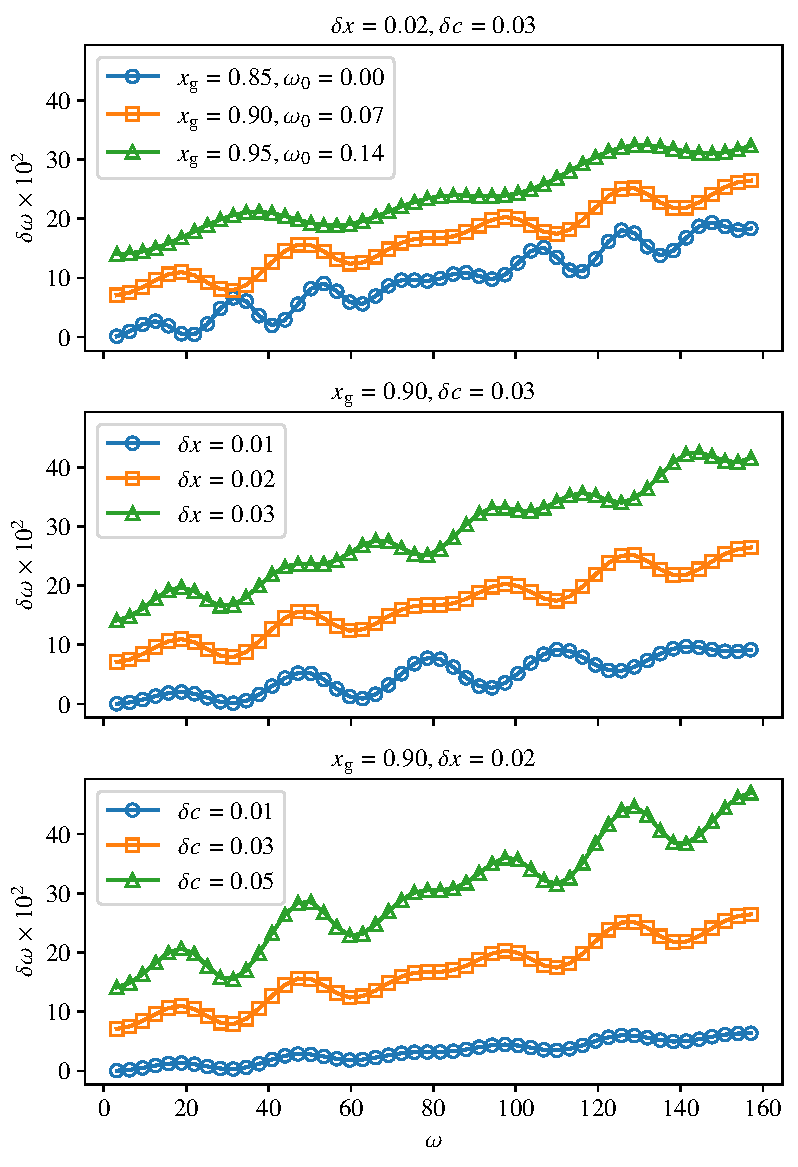
\includegraphics{figures/glitch-1d-example-results.pdf}
    \caption{The change in mode frequency induced by a change in sound speed of \(\delta c\) from \(x_0 - \delta x\) to \(x_0 + \delta x\) in a one-dimensional medium, bound such that \(x \in [0, 1]\) (see Figure \ref{fig:1d-diagram}). Outside of the perturbation the speed of sound, \(c=1\).
    The frequencies in the top panel are offset by \(\omega_0\).
    Points are joined by straight lines to guide the eye.
    }
    \label{fig:1d-results}
\end{figure}

%This may be interpreted as the nodes of each standing wave passing in and out of region 2 with increasing \(n\). Where there is a node, the wave is least sensitive to a change in structure, and 

The small phase offset \(\epsilon\) in Equation \ref{eq:1d-phase} is required for the wave function to satisfy the boundary conditions at \(x = 0\). However, adding \(\epsilon\) shifts the effective location of \(x_0\) --- it changes the scale of the \(x\)-axis by a factor of \((1 + \epsilon)\). We plot \(\epsilon\) against \(\omega\) in Figure \ref{fig:1d-phase} and show that its magnitude is \(\sim 10^{-4}\), much smaller than the location and size of region 2. The oscillation caused by the glitch also shows up in Figure \ref{fig:1d-phase}, with its properties affected in a similar way to Figure \ref{fig:1d-results}.

\begin{figure}
    \centering
    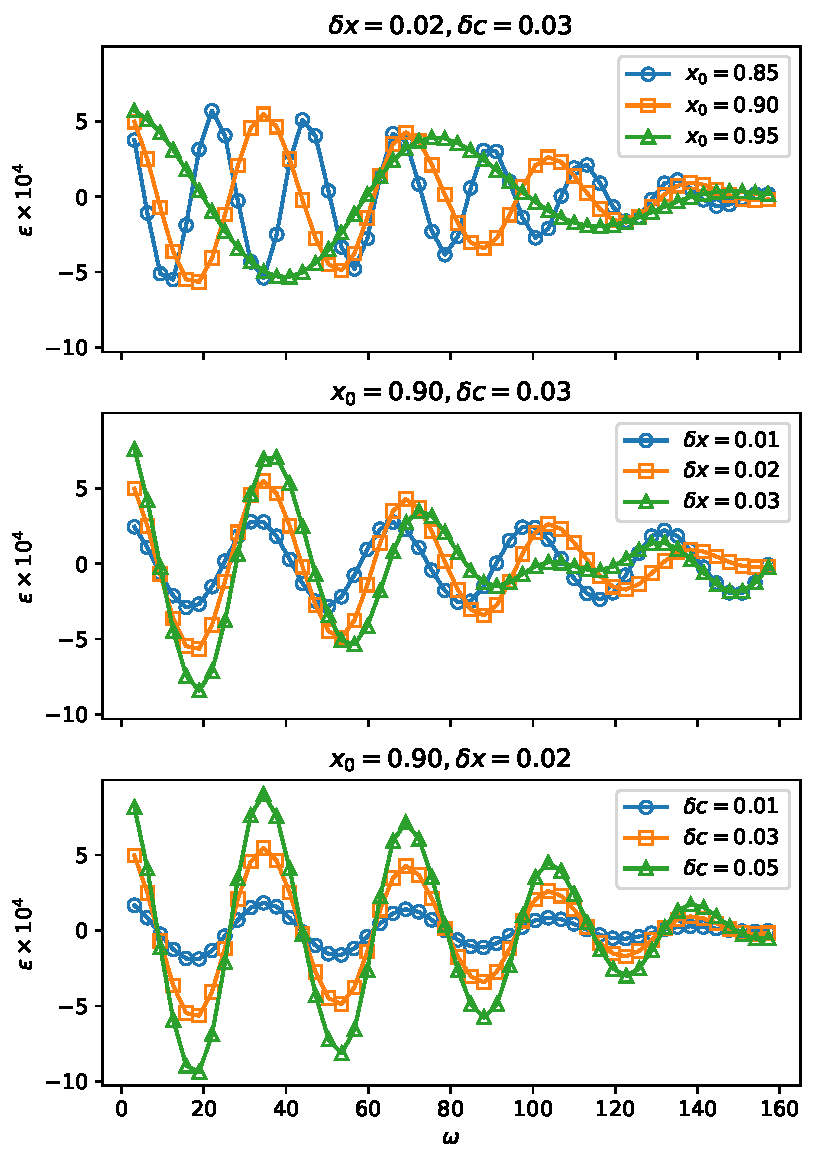
\includegraphics{figures/glitch-1d-example-phase.pdf}
    \caption{The same as Figure \ref{fig:1d-results} but showing the phase offset \(\epsilon\) required to satisfy the boundary conditions.}
    \label{fig:1d-phase}
\end{figure}

Finding an approximate solution for \(\delta\omega\) is beyond the scope of this simple example. However, we can show that by modelling \(\delta\omega\), we can recover information about the structural glitch. Let us build a model \(\delta\omega = f(\omega)\). Looking at Figure \ref{fig:1d-results}, we propose a form for \(f\),
%
\begin{equation}
    f(\omega) = a_1 \omega - a_2 \sin (\tau_1 \omega) \cos (\tau_2 \omega), \label{eq:1d-domega-func}
\end{equation}
%
where \(a_1\) and \(a_2\) are coefficients which are both functions of \(\delta x\) and \(\delta c\). Parameters \(\tau_1\) and \(\tau_2\) are the `frequencies' (units of time\footnote{A frequency in \(\omega\) would have units of time, but shouldn't be confused with a periodicity in \(\omega\).}) of oscillations in \(\delta\omega\), which are functions of \(\delta x\) and \(x_0\) respectively.

We fit Equation \ref{eq:1d-domega-func} to \(\delta\omega_n\) obtained from a glitch located at \(x_0 = 0.9\), with half-width \(\delta x = 0.02\), and change in sound speed \(\delta c = 0.03\). The best fitting line is shown in Figure \ref{fig:1d-fit}. We will see that \(\tau_1 \simeq 2\delta\tau\), where \(\delta\tau\) is half the acoustic width of the glitch --- the time at which sound takes to transverse the region. The second `frequency' \(\tau_2 \simeq 2\tau_0\), where \(\tau_0\) is the sound travel time from the nearest edge to the centre of the glitch, \(x_0\). Since the speed of sound \(c(x) \approx 1\) throughout the medium, \(x_0 \simeq L - \tau_0\). Our example fit yields \(\tau_1 \approx \SI{0.0389}{\second\per\radian}\) and \(\tau_2 \approx \SI{0.199}{\second\per\radian}\), approximately recovering the input glitch half-width of \num{0.02} and location of \num{0.9}.

\todo{Repeating this for different glitch parameters,  how the `frequencies' \(\tau_1\) and \(\tau_2\) relate to the half-width and location of the glitch respectively.}

% NOTE: Could take this further to show a1 = 2 dc dtau / L and a2 = dc / L

\begin{figure}
    \centering
    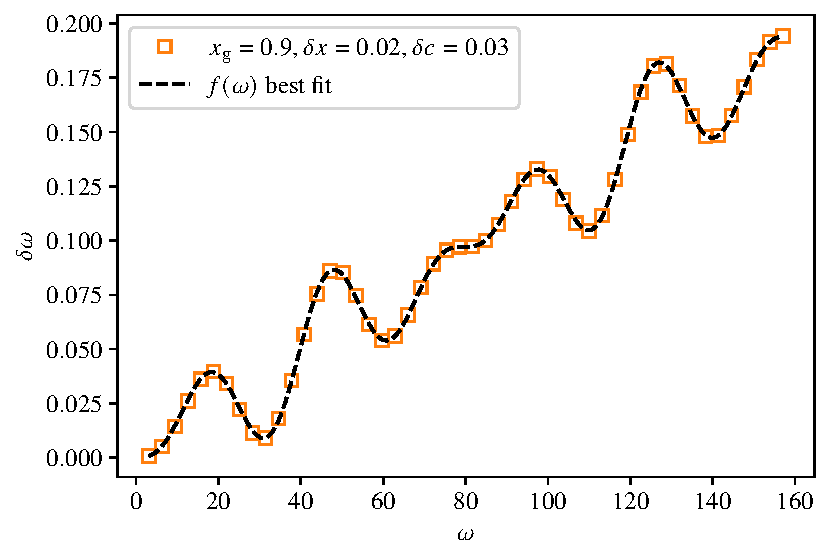
\includegraphics{figures/glitch-1d-fit.pdf}
    \caption{Best fit of Equation \ref{eq:1d-domega-func} to \(\delta\omega_n\) for \(n=1,\dots,50\), \(L=1\), and \(c=1\).}
    \label{fig:1d-fit}
\end{figure}

It would not be hard to believe that a similar oscillation could be found in the mode frequencies of a star, although its structure is more complicated. We showed that fitting to \(\delta\omega\) we may can recover properties of a glitch. In the next section, we will build upon this analogy and explore acoustic glitches in stars.

% NOTES: Go slowly through this. The next step is to fit a simple mode to theses oscillations and show that we can find x0 and dx. And show how the amplitude scales with dc.

% NOTES: When it comes to fitting the helium glitch, consider first fitting a GP to the modes with a free noise term. Fix the kernel scale to a series of values and show that we can see the glitch in the residuals. Of course, this leaves the question of what kernel scale to use. Well, we could just model everything at once!

\section[Glitches in stars]{Acoustic glitches in solar-like oscillators}

In the previous section, we considered a glitch in a homogeneous medium, where the speed of sound is constant everywhere else. In a star, the adiabatic sound speed is not constant. It depends on the density (\(\rho\)) and pressure (\(P\)),
%
\begin{equation}
    c^2 = \gamma \frac{P}{\rho},
\end{equation}
%
where \(\gamma \equiv \Gamma_1\) is the first adiabatic exponent,
%
\begin{equation}
    \gamma = \left( \frac{\partial \ln P}{\partial \ln \rho} \right)_S,
\end{equation}
%
at constant entropy, \(S\). Chandrasekhar introduced three adiabatic exponents (\(\Gamma_1,\Gamma_2,\Gamma_3\)) to describe the non-ideal gas inside a star \needcite{}. In this chapter, we do not use the other two and hence refer the first as \(\gamma\).

For the most part, \(\gamma\), \(P\), and \(\rho\) change smoothly with radius inside a star. However, a small structural glitch in these quantities would lead to a sudden change in sound speed. In the previous section, we showed how such a perturbation can lead to an oscillation in the eigenfrequencies of pressure waves in a homogeneous medium. Characterising this oscillation allowed us to measure the properties of the glitch. If similar glitches were present in a star, then we might be able to do the same. In this section, we explore the origins of glitches inside a solar-like star. Then, we see what effect these have on the eigenfrequencies, a quantity we can measure through asteroseismology.

Firstly, let us consider the sound speed profile of a Sun-like star. Particularly, we want to see how the sound speed changes on the timescale of a pressure wave moving through the star. As discovered in Section \ref{sec:1d-glitch}, a convenient timescale to work with is the acoustic depth, \(\tau\). Here, we define \(\tau_\star\) as the time taken for a pressure wave to travel from its surface (\(r=R\)) to some radius \(r_\star\) under the assumption of spherical symmetry,
%
\begin{equation}
    \tau(r_\star) = \int_R^{r_\star} \frac{\dd r}{c(r)} \equiv \tau_0 - \int_0^{r_\star} \frac{\dd r}{c(r)},\label{eq:tau}
\end{equation}
%
where the acoustic radius of the star\footnote{Not to be confused with the glitch location, \(\tau_0\), in Section\ref{sec:1d-glitch}.}, \(\tau_0 = \tau(0)\), relates approximately to the average large frequency separation \(\langle\Delta\nu_{nl}\rangle^{-1} \simeq 2\tau_0\).

In Figure \ref{fig:sound-speed-gradient}, we show the sound speed gradient with respect to \(\tau\) for model S \todo{Define model S in a previous chapter}. We see how the speed of sound changes smoothly throughout the star. In the convective envelope, where p-modes propagate, there is a noticeable wiggle around \SI{700}{\second} and a sharp change in direction at its base. The first is caused by the ionisation of helium, which affects \(\gamma\) by increasing the number of free electrons and thus modifying the free energy of the gas. We explore this further in Section \ref{sec:helium-glitch}. The second is due to a discontinuity in the second temperature gradient as the structure moves from convectively unstable to radiative, which will be discussed in Section \ref{sec:bcz-glitch} \todo{Put a few references here of work which has studied these before}.

\begin{figure}
    \centering
    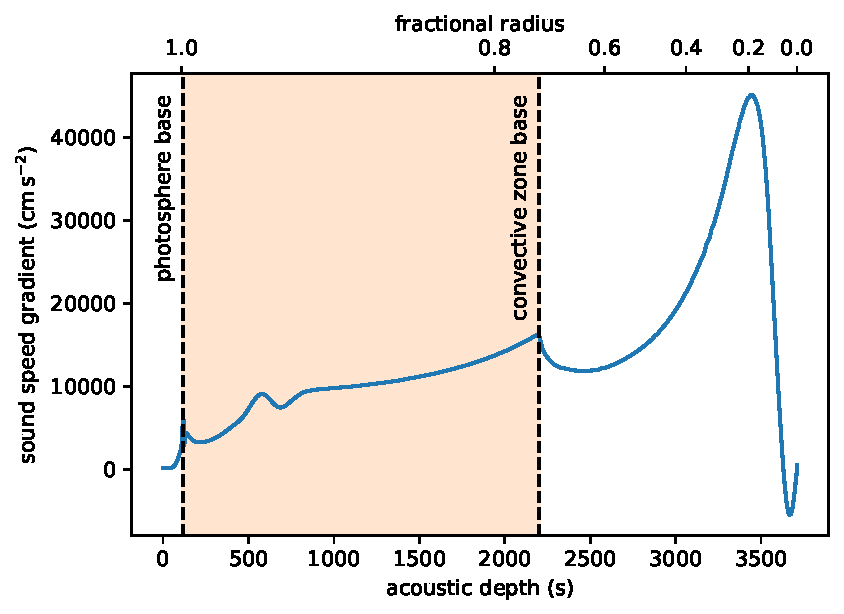
\includegraphics{figures/sound-speed-gradient.pdf}
    \caption{The sound speed gradient (\(\dd c/\dd \tau\)) of model S plot against the acoustic depth (\(\tau\)). The fractional radius to the photosphere base is given on the top axis. The convective envelope is shaded and the bases of the photosphere and convective zone are marked with dashed lines.}
    \label{fig:sound-speed-gradient}
\end{figure}

\subsection{Helium ionisation glitch}\label{sec:helium-glitch}

In this section, we will first show how the sound speed inside a solar-like star is affected by the ionisation of hydrogen and helium. Then, we will see that an increase in helium abundance increases the effect of helium ionisation on the speed of sound. Starting with the variational principle, we derive a commonly used form of the glitch signature found in the mode frequencies. In the process, we show that the oscillation modes are sensitive to changes in sound speed near the surface.

The speed of sound in the star is proportional to \(\gamma\). As a chemical species in the star ionises, the number of particles and thus chemical potential of the species changes. This induces a gradient in the thermal free energy of the gas which relates to the pressure and entropy of the gas. Therefore, we expect ionisation to cause a change in the pressure-density gradient at constant entropy, \(\gamma\). Using an approximate form for the first adiabatic exponent from \citet{Houdayer.Reese.ea2021}, we show how \(\gamma\) is affected by the ionisation of helium and hydrogen in Figure \ref{fig:gamma-zones}. We see that hydrogen ionisation has the largest effect on \(\gamma\) close to the surface of the star. The first and second ionisations of helium occur deeper in the star, at higher temperatures. We can see that the second ionisation of helium has a greater affect on \(\gamma\) than the first. This is because the ionisation energy of He\,\textsc{ii} is higher than He\,\textsc{i} and the ground state degeneracy of He\,\textsc{ii} is less than He\,\textsc{i}.

\begin{figure}
    \centering
    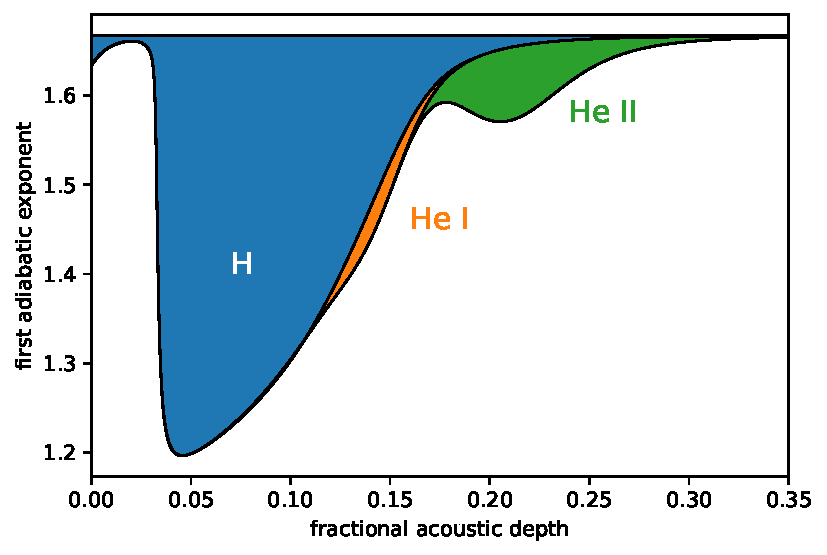
\includegraphics{figures/adiabatic-ionisation-regions.pdf}
    \caption{The depressions in the first adiabatic exponent (\(\gamma\)) caused by the ionisation of hydrogen (H), and the first and second ionisations of helium (He\,\textsc{i} and He\,\textsc{ii}). The x-axis is the fractional acoustic depth from the surface of the star, \(\tau/\tau_0\).}
    \label{fig:gamma-zones}
\end{figure}

Let us consider a star of mass \(M\) with hydrogen and helium mass fractions of \(X\) and \(Y\) respectively. To demonstrate the effect of ionisation and stellar structure on \(\gamma\), we will use equations from \citet{Houdayer.Reese.ea2021} to approximate \(\gamma\) in a solar-like star as a function of temperature and density,
%
\begin{equation}
    \gamma \simeq \frac{5}{3} - \frac{2}{3} \, \eta(T, \rho), \label{eq:gamma1}
\end{equation}
%
where \(\eta\) represents the depression in \(\gamma\). Considering a hydrogen-helium mixture where \(X + Y \approx 1\), \(\eta\) is given by \citep[cf.][]{Houdayer.Reese.ea2021},
%
\begin{equation}
    \begin{split}
        \eta(T, \rho) &= \frac{1}{\partial_{TT}^2 f} \left[n_\hydrogen y_\hydrogen \, (1 - y_\hydrogen) \, \frac{(\chi_\hydrogen / k_B T)^2}{2 - y_\hydrogen}
        % \right. \\ &\left. 
        + n_\helium y_\helium^{(1)} \left(1 - y_\helium^{(1)}\right) \left(\frac{\chi_\helium^{(1)}}{k_B T}\right)^2 
        \right. \\ &\left.
        + \, n_\helium y_\helium^{(2)} \left(1 - y_\helium^{(2)}\right) \left(\frac{\chi_\helium^{(2)}}{k_B T}\right)^2\right],
    \end{split}
\end{equation}
%
where \(k_B\) is the Boltzmann constant. The parameter \(\partial_{TT}^2\) is the second partial derivative of the free energy density with respect to temperature (\(T\)),
%
\begin{equation}
    \begin{split}
        \partial_{TT}^2 f &\simeq \frac{3}{2} + n_\hydrogen y_\hydrogen \left[ \frac{3}{2} + \frac{(1 - y_\hydrogen)}{2 - y_\hydrogen} \left(\frac{3}{2} + \frac{\chi_\hydrogen}{k_B T}\right)^2 \right] %\\
        + n_\helium y_\helium^{(1)} \left[ \frac{3}{2} + \left(1 - y_\helium^{(1)}\right) \left(\frac{3}{2} + \frac{\chi_\helium^{(1)}}{k_B T}\right)^2 \right] \\
        &+ n_\helium y_\helium^{(2)} \left[ \frac{3}{2} + \left(1 - y_\helium^{(2)}\right) \left(\frac{3}{2} + \frac{\chi_\helium^{(2)}}{k_B T}\right)^2 \right],
    \end{split}
\end{equation}
%
where \(n_\mathbb{X} = N_\mathbb{X} / N\) is the number density and \(\chi_\mathbb{X}^{i}\) is the \(i\)-th ionisation energy of species \(\mathbb{X}\). Parameter \(y_\mathbb{X}^i\) is related to a reduced form of Saha's equation \needcite,
%
\begin{equation}
    \frac{(y_\mathbb{X}^i)^q}{1 - y_\mathbb{X}^i} = \frac{2 g_\mathbb{X}^i}{g_\mathbb{X}^{i-1}} \frac{\overline{m}}{\rho \lambda_\ee^3} \, \ee^{- \chi_\mathbb{X}^i / k_B T},
\end{equation}
%
where \(q = 2\) for hydrogen, \(q = 1\) for helium, \(\overline{m} = M/N\) is the mean mass, and \(g_\mathbb{X}^i\) is the ground-state degeneracy of ionisation state \(i\). We used these equations to produce Figures \ref{fig:gamma-zones} and \ref{fig:gamma-temp-density}.

In Figure \ref{fig:gamma-temp-density} we plot \(\gamma\) as a function of pressure and temperature. The first panel illustrates the three ionisation regions of hydrogen and helium. The value of \(\gamma\) decreases when the ionisation reaction is occurring. The magnitude of the effect depends primarily on the temperature-density profile of the star. Additionally, in the second panel we see that an increase in helium abundance decreases \(\gamma\) in the helium ionisation regions. A temperature-density profile from model S is shown to see how the star probes the ionisation regions. We can imagine a hotter star shifting this line such that ionisation occurs closer to the surface. Similarly, the effect on \(\gamma\) would be smaller in denser star. Although helium abundance dominates the effect on \(\gamma\), there is still some dependence on other stellar quantities.

\begin{figure}
    \centering
    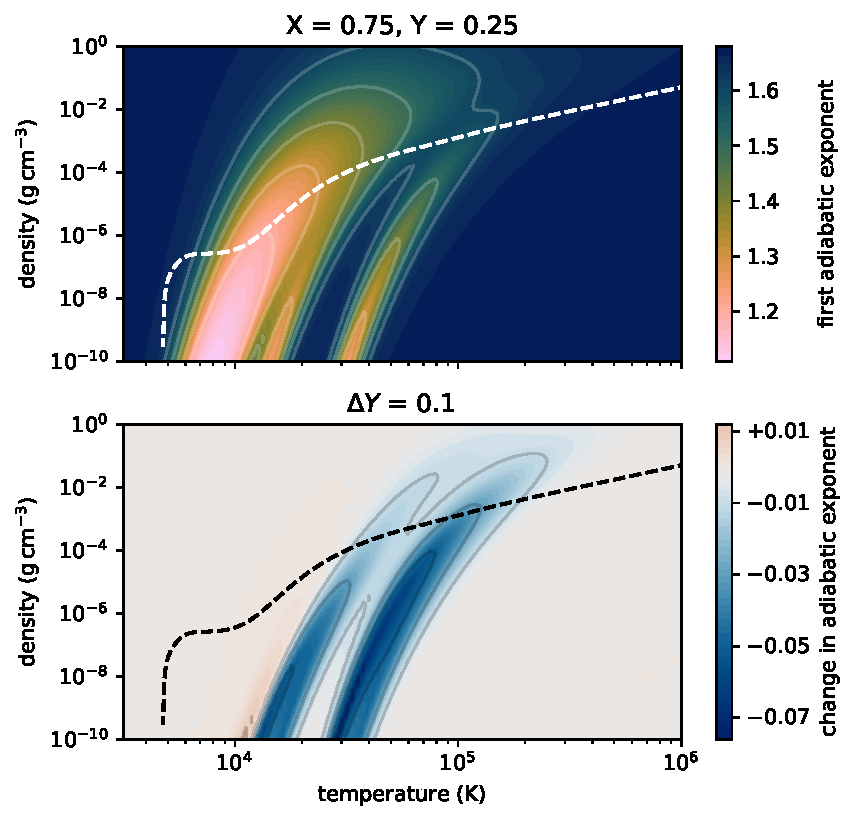
\includegraphics{figures/adiabatic-ionisation-temp.pdf}
    \caption{Temperature-density profile of a Sun-like star. \emph{Top:} The first adiabatic exponent \(\gamma\) as a function of temperature and density, calculated using Equation \ref{eq:gamma1} for a helium mass fraction, \(Y=0.25\). \emph{Bottom:} The change in \(\gamma\) induced by a change in helium abundance, \(\Delta Y = 0.1\). In both panels, the dashed line shows the temperature-density profile of model S.}
    \label{fig:gamma-temp-density}
\end{figure}

To show the effect of small changes in \(\gamma\) on the sound speed, we plot the sound speed gradient in Figure \ref{fig:gamma-sound-speed}. The three models shown were evolved to the same central temperature with different initial helium abundances. The dominant effect of helium abundance appears as a Gaussian-like depression in \(\gamma\) around the second ionisation of helium. We see how larger helium abundance increases the width and depression in \(\gamma\), which is reflected in the sound speed gradient. A larger \(Y\) also leads to a relative reduction in hydrogen abundance. This slightly shrinks the width of the hydrogen ionisation region.

\begin{figure}
    \centering
    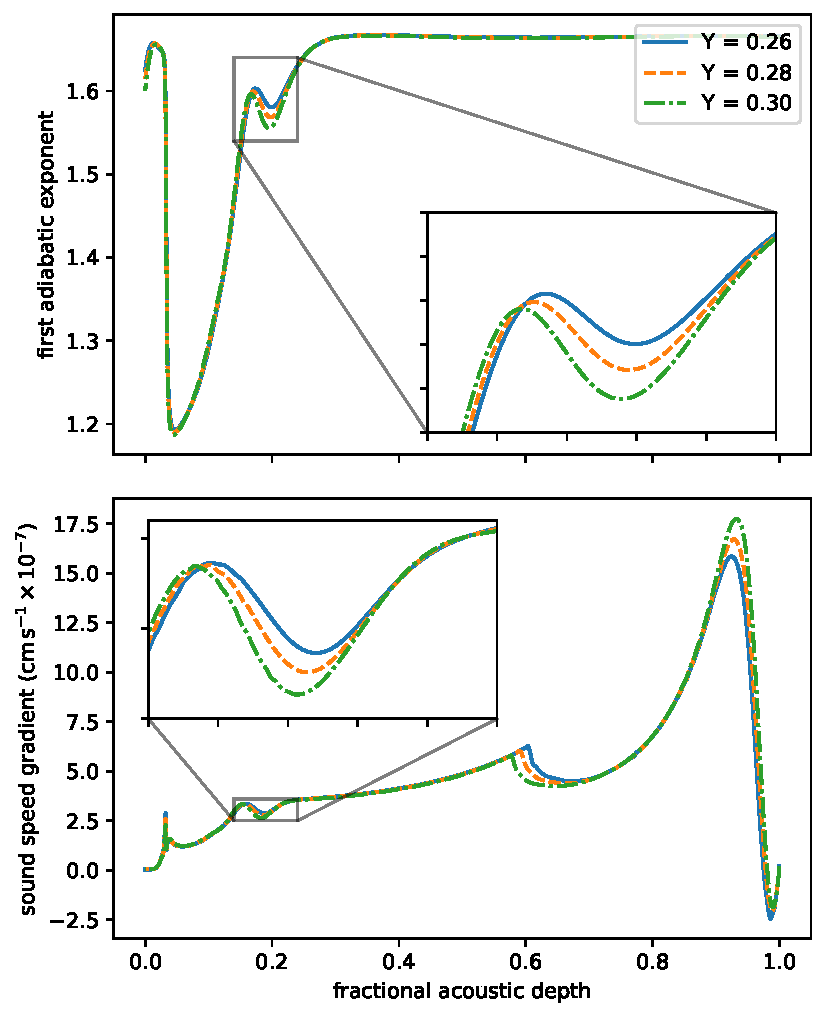
\includegraphics{figures/helium-ionisation-sound-speed.pdf}
    \caption{The effect on the sound speed profile for three solar-like stars with initial helium mass fractions of 0.26 (\emph{solid}), 0.28 (\emph{dashed}), and 0.3 (\emph{dot-dashed}). The models were each evolved to a central helium mass fraction of 0.6. \emph{Top:} The first adiabatic exponent \(gamma\). \emph{Bottom:} The sound speed gradient \(\dd c/\dd t\) where \(t = \tau/\tau_0\) is the fractional acoustic depth (plot on the x-axis).}
    \label{fig:gamma-sound-speed}
\end{figure}

To see how a change in \(\gamma\) affects the mode frequencies, we will consider the sensitivity of a given mode to structural changes in the star. We can get there by starting with the variational principle \citep{Chandrasekhar1964},
%
\begin{equation}
    \omega^2 = \frac{\mathcal{E}}{\mathcal{I}}\label{eq:var-prin}
\end{equation}
%
which approximates the characteristic frequencies of a spherically symmetric, slowly rotating star as a function of the mode inertia,
%
\begin{equation}
    \mathcal{I} = \int_0^R \vect{\xi} \cdot \vect{\xi} \, \rho r^2 \, \dd r
\end{equation}
%
and \(\mathcal{E}\) which is proportional to the mode energy,
%
\begin{equation}
    \mathcal{E} = \int_0^R \left[\gamma P (\dive{\vect{\xi}})^2 + 2(\vect{\xi}\cdot \nabla P) \dive{\vect{\xi}} + (\vect{\xi}\cdot \nabla P) (\vect{\xi}\cdot\nabla\ln\rho)\right] r^2 \, \dd r.
\end{equation}
%
These equations depend on \(\vect{\xi}\), the Lagrangian perturbation vector of the pulsation mode (the amplitude and direction of the wave). \todo{Explain the meaning of each term}. A structural glitch in the star would cause a small change in frequency (\(\delta\omega\)). Differentiating both sides of Equation \ref{eq:var-prin} with respect to \(\omega\), we get,
%
\begin{align}
    2\omega &= \frac{1}{\mathcal{I}} \left( \frac{\delta\mathcal{E}}{\delta\omega} - \omega^2 \frac{\delta\mathcal{I}}{\delta\omega}\right), \qquad \left[\times \frac{\delta\omega}{2\omega^2}\right] \notag \\
    \frac{\delta\omega}{\omega} &= \frac{1}{2\,\mathcal{I}} \left(\frac{\delta\mathcal{E}}{\omega^2} - \delta\mathcal{I}\right).
\end{align}
%
The perturbations \(\delta\mathcal{E}\) and \(\delta\mathcal{I}\) depend on changes in the state variables. To see the effect of a change i on the modes, it is possible to rewrite this as a function of the so-called structural kernels \(\mathcal{K}_{a,b}\), for example,
%
\begin{equation}
    \frac{\delta\omega}{\omega} = \int_0^R \left(\mathcal{K}_{c^2,\rho} \frac{\delta c^2}{c^2} + \mathcal{K}_{\rho,c^2} \frac{\delta \rho}{\rho} \right) \dd r.\label{eq:kernels}
\end{equation}
%
where \(\mathcal{K}_{a, b}\) gives the relative effect on \(\omega\) due to a perturbation in a state variable \(a\) at fixed \(b\), at a given \(r\). These kernels are defined fully in \citet{Gough.Thompson1991}.

We plot the kernels in Figure \ref{fig:kernels} for a few modes. Both decay through the star, meaning that the modes are less sensitive to structural changes deeper in the star. \todo{Explain why this is, from asymptotic theory frequencies determined by sound speed}. We see that for high-order modes, the second term of Equation \ref{eq:kernels} approximately integrates to zero, unless there is a sharp change in \(\delta\rho/\rho\) (such as at the base of the convective zone). Therefore, we may rewrite the 

%
\begin{equation}
    \frac{\delta\omega}{\omega} \simeq \int_0^R \mathcal{K}_{\gamma,\rho} \frac{\delta\gamma}{\gamma} \dd r,\label{eq:delta-omega}
\end{equation}
%
where \(\mathcal{K}_{\gamma,\rho} \equiv \mathcal{K}_{c^2,\rho}\) is shown in \citet{Gough1993} to satisfy,
%
\begin{equation}
    \omega^2 \mathcal{I}\mathcal{K}_{\gamma,\rho} = \frac12 \gamma P (\dive{\vect{\xi}})^2 r^2.\label{eq:gamma-kernel}
\end{equation}
%
show how this gets to, using equations for \(\xi_r\) and pressure perturbation \(P'\) from eq. 24-25 of e.g. \citet{Shibahashi1979}, \(\vect{\xi} = \xi_r \hat{r} + \vect{\xi}_h\) for high-order acoustic modes (where we can ignore the horizontal component of \(\vect{\xi}\)).
%
\begin{equation}
    \xi_r \simeq \frac{\psi_0}{r}\sqrt{\frac{K}{\rho}} \cos\psi,\qquad
    (\dive{\vect{\xi}})^2 \simeq \frac{\psi_0^2 \omega^3}{\gamma P c r^2} \sin^2\psi, \label{eq:xi-approx}
\end{equation}
%
where \(\psi_0\) is a proportionality constant and the radial wave number \(K \simeq \omega / c\) for high-order acoustic modes. The phase term \(\psi \simeq \omega \tau + \epsilon\) when \(\tau\) is not close to the upper turning point (where the wave is reflected near the stellar surface), and the small offset \(\epsilon\) is a slowly varying function of \(\tau\).

\begin{align}
    \mathcal{I} &\simeq \int_0^R \xi_r^2 \rho r^2 \, \dd r \notag\\
    &\simeq \psi_0^2 \int_0^R K \cos^2\psi \, \dd r \notag \\
    &= \frac12 \omega \psi_0^2 \int_0^R (1 + \cos 2 \psi) \frac{\dd r}{c}
\end{align}
%
Changing to an integral over acoustic depth we can evaluate it for high-order modes where \(\omega_n \ll \tau_0^{\,-1}\),
%
\begin{align}
    \mathcal{I} &\simeq \frac12 \omega \psi_0^2 \int_0^{\tau_0} [1 + \cos 2 (\omega\tau + \epsilon)] \, \dd \tau \simeq \frac12 \omega \psi_0^2 \tau_0.
\end{align}
%
Finally, substituting Equations \ref{eq:gamma-kernel} and \ref{eq:xi-approx} into Equation \ref{eq:delta-omega}, we get,
%
\begin{align}
    \frac{\delta\omega}{\omega} &\simeq \frac{1}{2\omega^2\mathcal{I}} \int \delta\gamma P (\dive{\vect{\xi}})^2 r^2 \, \dd r, \notag \\
    &\simeq \frac{\omega \psi_0^2}{2 \mathcal{I}} \int \frac{\delta\gamma}{\gamma}\sin^2\psi\frac{\dd r}{c}, \notag \\
    &= \frac{\omega \psi_0^2}{4 \mathcal{I}} \int \frac{\delta\gamma}{\gamma}(1 - \cos 2\psi)\frac{\dd r}{c}.
\end{align}
%
where the integral need only be evaluated in the region where \(\delta\gamma / \gamma\) is non-zero. We can see that \(\delta\omega\) is split into a smooth and an oscillating component. The smooth component may be treated later, but for now we focus on the oscillating part of \(\delta\omega\). Substituting for \(\mathcal{I}\) and \(\psi\), changing to an integral over acoustic depth we get,
%
\begin{equation}
    \left.\frac{\delta\omega}{\omega}\right|_\mathrm{osc} \simeq - \frac{1}{2\tau_0} \int \frac{\delta\gamma}{\gamma} \cos 2 (\omega\tau + \epsilon) \, \dd \tau,
\end{equation}
%

We have shown that a perturbation in \(\gamma\) can induce an oscillation in \(\omega\). The functional from of this oscillation depends on \(\delta\gamma/\gamma\). As shown in Figures \ref{fig:gamma-zones} and \ref{fig:gamma-temp-density}, the dominant perturbation due to a change in helium abundance is from the second ionisation of helium. There have been different attempts to approximate \(\delta\gamma/\gamma\,|_\heII\) in the literature, for example using a Dirac delta function or a triangular function \citep{Monteiro.Christensen-Dalsgaard.ea1994, Monteiro.Thompson2005}. In recent years, work modelling the glitch has used the formulation from \citet{Houdek.Gough2007} where the perturbation is modelled with a Gaussian shape,
%
\begin{equation}
    \left.\frac{\delta\gamma}{\gamma}\right|_\heII \simeq - \frac{\Gamma_\heII}{\Delta_\heII \sqrt{2\pi}} \, \ee^{- \frac12{(\tau - \tau_\heII)^2}/{\Delta_\heII^2} }, \label{eq:he-gamma}
\end{equation}
%
where \(\Gamma_\heII\) is the area, \(\Delta_\heII\) is the characteristic width, and \(\tau_\heII\) is the center of the ionisation region.

Combine the above two equations with a change of variables to \(x = (\tau - \tau_\heII)/\Delta_\heII\), we get,
%
\begin{equation}
    \left.\frac{\delta\omega}{\omega}\right|_{\heII, \mathrm{osc}} \simeq \frac{\Gamma_\heII}{2\sqrt{2\pi} \, \tau_0} \, \int_{-\infty}^\infty \ee^{- x^2/2} \cos 2 (\Delta_\heII \omega x + \widetilde{\epsilon_\heII}) \, \dd x
\end{equation}
%
where \(\widetilde{\epsilon_\heII} = \omega\tau_\heII + \epsilon_\heII\) and the phase \(\epsilon=\epsilon_\heII\) is assumed constant accross the glitch region. We can solve the above integral analytically using differentiation under the integral sign by introducing an arbitrary variable \(a\),
%
\begin{equation}
    I(a) = \int_{-\infty}^\infty \ee^{- x^2/2 } \cos 2 (\Delta_\heII \omega x a + \widetilde{\epsilon_\heII}) \, \dd x
\end{equation}
%
Differentiating this with respect to \(a\), and then integrating by parts gets,
%
\begin{align}
    I'(a) &= - 2 \Delta_\heII \omega \int_{-\infty}^\infty x \, \ee^{- x^2/2 } \sin 2 (\Delta_\heII \omega x a + \widetilde{\epsilon_\heII}) \, \dd x, \notag\\
    &= - 2 \Delta_\heII \omega \int_{-\infty}^\infty \sin 2 (\Delta_\heII \omega x a + \widetilde{\epsilon_\heII}) \, \dd \ee^{- x^2/2 }, \notag\\
    &= 2 \Delta_\heII \omega \left\{ \left[ \ee^{- x^2/2 } \sin 2 (\Delta_\heII \omega x a + \widetilde{\epsilon_\heII}) \right]_{-\infty}^\infty - 2 \Delta_\heII \omega a \int_{-\infty}^\infty \ee^{- x^2/2 } \cos 2 (\Delta_\heII \omega x a + \widetilde{\epsilon_\heII}) \, \dd x \right\}, \notag\\
    &= - 4 \Delta_\heII^2 \omega^2 a \, I(a),
\end{align}
%
which is a differential equation with the solution,
%
\begin{equation}
    \begin{split}
        I(a) = I(0) \ee^{- 2 \Delta_\heII^2 \omega^2 a^2}, \qquad I(0) &= \int_{-\infty}^\infty \ee^{- x^2/2 } \cos 2 \widetilde{\epsilon_\heII} \, \dd x, \\
        &= \sqrt{2\pi} \, \cos 2 \widetilde{\epsilon_\heII},
    \end{split}
\end{equation}
%
Therefore, if we set \(a = 1\) for the case of the integral in Equation \ref{} we get the following for the oscillatory glitch signature \citep[cf.][]{Houdek.Gough2007},
%
\begin{equation}
    \left.\frac{\delta\omega}{\omega}\right|_{\heII, \mathrm{osc}} \simeq \frac{\Gamma_\heII}{2 \tau_0} \ee^{- 2 \Delta_\heII^2 \omega^2} \cos 2 (\tau_\heII\omega + \epsilon_\heII),
\end{equation}
%
To get this in a more familiar form in terms of cyclic frequency \citep[e.g.][]{Verma.Faria.ea2014,Verma.Raodeo.ea2017}, we substitute \(\omega = 2\pi\nu\),
%
\begin{equation}
    \left.\frac{\delta\nu}{\nu}\right|_{\heII, \mathrm{osc}} \simeq \nu_0 \Gamma_\heII \, \ee^{- 8 \pi^2 \Delta_\heII^2 \nu^2} \, \sin ( 4 \pi \tau_\heII \nu + \phi_\heII),
\end{equation}
%
where \(\phi_\heII = 2(\epsilon_\heII + \pi/4)\), and \(\nu_0 = (2 \tau_0)^{-1}\) is the inverse acoustic diameter of the star.

\subsection{Base of the convective zone glitch}\label{sec:bcz-glitch}

The sensitivity of p-modes to glitches gets smaller further into the star. However, we should not neglect the effect of a discontinuity at the base of the convective zone. This arises 

\begin{figure}
    \centering
    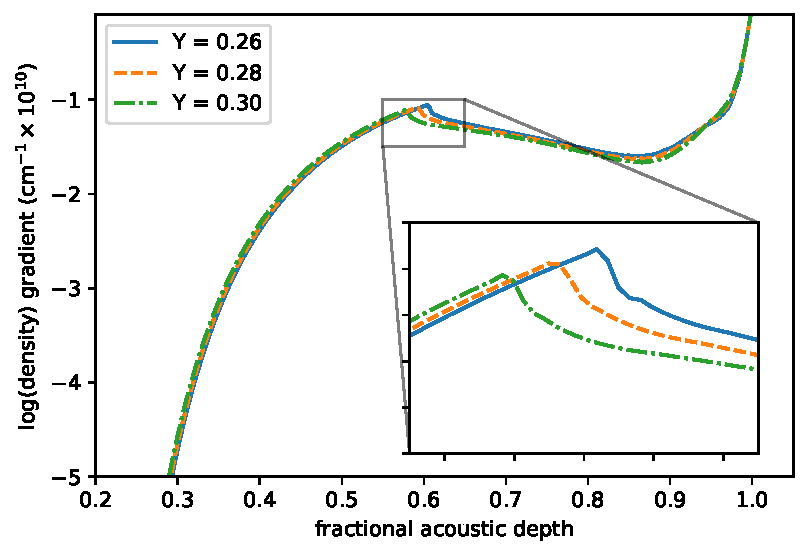
\includegraphics{figures/bcz-density-gradient.pdf}
    \caption{Discontinuity in the density gradient at the base of the convective zone for three solar-like stars with initial helium mass fractions of 0.26 (\emph{solid}), 0.28 (\emph{dashed}), and 0.3 (\emph{dot-dashed}).}
    \label{fig:bcz-density}
\end{figure}


We can take a similar approach to the previous section but now considering the second kernel \(\mathcal{K}_{\rho,c^2}\) in Equation \ref{eq:kernels}. However, \citet{Houdek.Gough2007} take another approach by considering the discontinuity as it appears in the acoustic cut-off frequency, \(\omega_{ac}\). The details of this derivation are beyond the scope of this work. We quote their result for the change in frequency induced by a density discontinuity at the base of the convective zone located at an acoustic depth of \(\tau_\bcz\),
%
\begin{equation}
    \left.\frac{\delta\omega}{\omega}\right|_{\bcz,\mathrm{osc}} \simeq \frac{c_\bcz^2\Delta_\bcz}{8\tau_0 \omega^3} \left(1 + {1}/{4\tau_0^2\omega^2}\right)^{-1/2} \cos\left[2(\tau_\bcz \omega + \epsilon_\bcz) + \tan^{-1}(2\tau_0\omega)\right]
\end{equation}
%
where \(\epsilon_\bcz\) is some phase which depends slowly on \(\omega\), \(c_\bcz\) is the speed of sound and,
%
\begin{equation}
    \Delta_\bcz = \left.\frac{\dd^2 \ln\rho}{\dd r^2}\right|_{+r_\bcz} - \left.\frac{\dd^2 \ln\rho}{\dd r^2}\right|_{-r_\bcz}
\end{equation}
%
is the change in second derivative of density at the base of the convective zone (\(r = r_\bcz\)).

For high-order modes, \(\tau_0 \omega \gg 1\) and thus \(\tan^{-1}(2\tau_0\omega) \simeq \pi/2\), and \((1 + {1}/{4\tau_0^2\omega^2})^{-1/2} \simeq 1\). Therefore, we can simplify this and write it in a more familiar form in terms of cyclic frequency,
%
\begin{equation}
    \left.\frac{\delta\nu}{\nu}\right|_{\bcz,\mathrm{osc}} \simeq \frac{c_\bcz^2\Delta_\bcz\nu_0}{32\pi^3 \nu^3} \sin(4\pi\tau_\bcz\nu + \phi_\bcz)
\end{equation}
%
where \(\phi_\bcz\) is some approximately constant phase term.

\section[Modelling the glitch]{Modelling glitches in stellar oscillations}

The p-mode frequencies (\(\nu_{nl}\)) for a slowly rotating star are given by some function of their radial order (\(n\)) and angular degree (\(l\)). This function is not exactly known, making the prediction and identification of mode frequencies difficult. Typically, oscillation modes are identified in an acoustic power spectra through the process of `peakbagging' \citep[e.g.][]{Nielsen.Davies.ea2021}. We find these modes using approximate relations for \(\nu_{nl}\) as a guide. For example, from asymptotic theory \citep{Tassoul1980},
%
\begin{equation}
    \nu_{nl} \simeq \left(n + {l}/{2} + \varepsilon\right) \nu_0\label{eq:asy}
\end{equation}
%
where \(\varepsilon\) is some small offset depending on the boundary conditions, and \(\nu_0\) is inverse of the sound travel time across the stellar diameter. We can approximately determine \(\nu_0\) because \(\nu_0 \simeq \langle \Delta\nu_{nl} \rangle\) where \(\Delta\nu_{nl}\) is the difference between modes of consecutive \(n\). Fitting this equation, or measuring \(\langle \Delta\nu_{nl} \rangle\) can at most hold information about the mean density of the star (from Equation \ref{eq:tau}). The modes can be further approximated by a polynomial with increasing order in \(n\) \citep[e.g.][]{Ulrich1986,Kjeldsen.Bedding.ea2005}, but the physical meaning of its coefficients become difficult to interpret.

We want to extend this model to include parameters which carry more information about the star. Particularly, we want to model the acoustic glitch signatures in \(\nu_{nl}\) which arise from helium ionisation and the base of the convective zone (BCZ). These will provide parameters which correlate with helium abundance and the sharpness of the convective zone boundary. We can then extend the hierarchical model in Chapter \ref{chap:hmd} to include these parameters and provide better constraints on helium enrichment in the stellar population. Ultimately, we aim to take the information contained in the mode frequencies of a star and reduce its dimensionality to a handful of fundamental parameters.

Let us propose a new model, \(f(n, l)\), which we can fit to \(\nu_{nl}\) obtained from peakbagging,
%
\begin{equation}
    f(n, l) = \tilde{\nu}_{nl} + \delta\nu \label{eq:general-glitch}
\end{equation}
%
where \(\tilde{\nu}_{nl}\) represents the smoothly varying component of the modes (background) and \(\delta\nu\) is the small change in frequency due to glitches (signal). We assume the glitches contained in \(\delta\nu\) are comparatively small and rapidly varying compared to \(\tilde{\nu}_{nl}\). For example, the smooth component,
%
\begin{equation}
    \tilde{\nu}_{nl} = \nu_0 \sum_{k=0}^{K} a_k^{(l)} n^k, \label{eq:poly}
\end{equation}
%
could be a \(K\)-th order polynomial with coefficients \(a_k^{(l)}\). Then, in principle, \(\delta\nu\) could contain any glitch functions expected for a given star. In the previous section, we found the functional form of \(\delta\nu\) arising from acoustic glitches in solar-like oscillators \(\delta\nu = \delta_\helium(\nu) + \delta_\bcz(\nu)\), where,
%
\begin{align}
    \delta_\helium(\nu) &= \alpha_\helium \nu_0 \nu \, \ee^{-\beta_\helium \nu^2} \sin(4\pi\tau_\helium\nu + \phi_\helium), \label{eq:he-glitch}\\
    \delta_\bcz(\nu) &= \alpha_\bcz \nu_0 \nu^{-2} \, \sin(4\pi\tau_\bcz\nu + \phi_\bcz). \label{eq:bcz-glitch}
\end{align}
%
The parameters \(\alpha_\helium \cong \Gamma_\heII\) and \(\beta_\helium \propto \Delta_\heII^2\) relate to the area and variance of the Gaussian-like depression in \(\gamma\) caused by the second ionisation of helium. We neglect contribution by the first ionisation of helium because it would be a smaller signal at a similar acoustic depth. The amplitude parameter for the BCZ glitch, \(\alpha_\bcz \propto \Delta_{\bcz}\) is proportional to the difference in the second density derivative at the base of the convective zone and has units of frequency squared. The approximate acoustic depths of second helium ionisation and the BCZ are given by \(\tau_\helium\) and \(\tau_\bcz\) respectively, and \(\phi\) represents an arbitrary phase constant.

Directly fitting the glitch this way has been done before \citep[e.g.][]{Verma.Faria.ea2014,Verma.Raodeo.ea2017}. However, there are drawbacks to using a polynomial for \(\tilde{\nu}_{nl}\). Whilst a polynomial with \(K = \infty\) can represent any function, this is completely impractical here. If \(K\) is too low, then it will not be flexible enough, biasing \(\delta\nu_\helium\) and \(\delta\nu_\bcz\). Yet, if \(K\) is too high, then it will over-fit and the glitch signal will be missed. Regularising the polynomial is one solution to over-fitting, but this adds extra parameters to tune. Finally, a finite polynomial represents only a small fraction of function space, leading to our model to be systematically biased to a particular functional form of \(\tilde{\nu}_{nl}\).

\defcitealias{Verma.Raodeo.ea2019}{V19}

In this work, we will compare the method from \citet[][hereafter V19]{Verma.Raodeo.ea2019} with a new method defined in this work. Our method will make use of a Gaussian Process to marginalise over our uncertainty in the functional form of \(f(n, l)\). In the next section, we introduce the data used in comparing the two methods. In Section \ref{sec:glitch-methods}, we define both modelling methods being compared. Finally, we apply the methods to the data and analyse their results in Section \ref{sec:glitch-results}.

\subsection{Data}\label{sec:glitch-data}

In this section, we briefly outline the data used to compare our new method with the \citetalias{Verma.Raodeo.ea2019} method. For simplicity, we only use observations of radial mode frequencies in this work. However, both models can be extended to use higher-order modes.

\begin{table}
    \centering
    \caption{Observations of radial mode frequency \(\nu_n\) at radial order \(n\) for model star S (\emph{left}) and 16 Cyg A (\emph{right}). \(N\) are the number of observed radial orders and the scale of the Gaussian noise added to each column is given by \(\sigma_\obs\) where appropriate. The values and their uncertainties for 16 Cyg A come from \citet{Lund.SilvaAguirre.ea2017}.}
    \label{tab:glitch-obs}
    \begin{tabular}{ccccc}
\toprule
Case & Worst & Better & Best & Truth \\
$N, \sigma_n$ & 6, 1.00 & 12, 0.10 & 18, 0.01 &  \\
$n$ &  &  &  &  \\
\midrule
12 & --- & --- & 1781.726 & 1781.729 \\
13 & --- & --- & 1914.348 & 1914.330 \\
14 & --- & --- & 2047.296 & 2047.314 \\
15 & --- & 2180.16 & 2180.107 & 2180.125 \\
16 & --- & 2312.00 & 2312.030 & 2312.029 \\
17 & --- & 2442.64 & 2442.807 & 2442.808 \\
18 & 2577.2 & 2574.32 & 2574.260 & 2574.263 \\
19 & 2706.4 & 2706.50 & 2706.612 & 2706.596 \\
20 & 2839.0 & 2839.46 & 2839.446 & 2839.476 \\
21 & 2971.5 & 2972.92 & 2972.718 & 2972.727 \\
22 & 3107.4 & 3105.77 & 3105.749 & 3105.759 \\
23 & 3240.0 & 3239.18 & 3239.177 & 3239.175 \\
24 & --- & 3372.94 & 3372.980 & 3372.990 \\
25 & --- & 3507.22 & 3507.115 & 3507.112 \\
26 & --- & 3641.56 & 3641.715 & 3641.702 \\
27 & --- & --- & 3776.339 & 3776.350 \\
28 & --- & --- & 3911.281 & 3911.279 \\
29 & --- & --- & 4046.319 & 4046.312 \\
\bottomrule
\end{tabular}

\end{table}

\begin{figure}
    \centering
    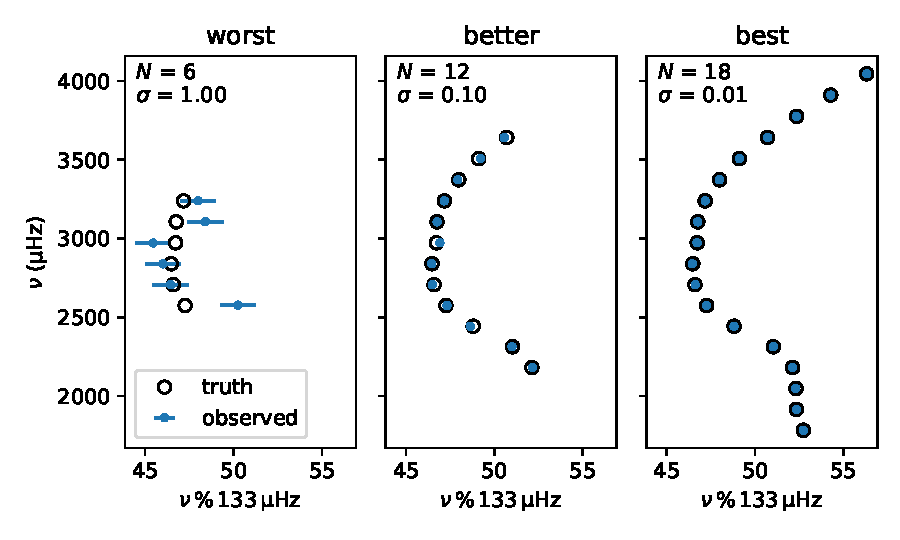
\includegraphics{figures/glitch-test-obs.pdf}
    \caption{Echelle plot of simulated true and `observed' radial mode frequency data from model star S for worst-, better-, and best-case scenarios.}
    \label{fig:glitch-test-obs}
\end{figure}
% \subsubsection{Test Star}

\paragraph{Test Star} We created three sets of test data for worst-, better-, and best-case scenarios using stellar model S to compare the two methods. We recall that stellar model S is similar to the Sun, with surface parameters of \(\teff = \SI{5682}{\kelvin}\), \(\log g = 4.426\) and \([\mathrm{Fe/H}] = 0.03\), and bulk parameters of \(M = \SI{1.00}{\solarmass}\), \(R = \SI{1.01}{\solarmass}\) and \(\mathrm{Age} = \SI{4.07}{\giga\year}\). We calculated radial order modes (\(\nu_{n,l=0} \equiv \nu_n\)) for the test star using the \textsc{GYRE} oscillation code \citep{Townsend.Teitler2013}. We then selected different numbers of modes (\(N\)) symmetrically about a reference frequency \(\nu_\mathrm{ref} = \SI{2900}{\micro\hertz}\) (close to the expected frequency at maximum power of the star). For each test case, we added differing amounts of Gaussian noise (scaled by \(\sigma_\obs\)) to the frequencies. The parameters and mode frequencies for each test case are shown in Table \ref{tab:glitch-obs} and the modes are plot in Figure \ref{fig:glitch-test-obs}. We can see the effect of the glitch in the echelle plots, where there is a large `wiggle' at low frequency. The effect of the glitch is present in the better case and clearest in the best case scenario.

% \subsubsection{16 Cyg}

\paragraph{16 Cyg A} We used the asteroseismic benchmark star 16 Cyg A as an example with which to compare glitch fitting methods. We adopted values for 16 radial mode frequencies identified by \citet{Lund.SilvaAguirre.ea2017} using observations from \emph{Kepler} \citep[KIC 12069424;][]{Borucki.Koch.ea2010}. The mode frequencies and their associated uncertainties are given in Table \ref{tab:glitch-obs}. The glitch has been previously studied for 16 Cyg A with its binary companion 16 Cyg B in \citet{Verma.Faria.ea2014}, making it a useful subject for comparison. Similarly to model S, this target is a solar analogue. However, it is slightly hotter, more evolved and more metal-rich, with \(\teff = \SI{5825(50)}{\kelvin}\), \(\log g = \SI{4.33(7)}{\dex}\) and \([\mathrm{Fe/H}] = \SI{0.10(3)}{\dex}\) \citep{Ramirez.Melendez.ea2009}. Its bulk stellar parameters are \(M \approx \SI{1.1}{\solarmass}\), \(R \approx \SI{1.2}{\solarradius}\) and \(\mathrm{Age} \approx \SI{7}{\giga\year}\) \citep{SilvaAguirre.Lund.ea2017}.

\subsection{Methods}\label{sec:glitch-methods}

In this section, we describe the two models for radial mode frequency, \(\nu_n = f(n, l=0)\), and their fitting methods being compared in this work. The first is the \citetalias{Verma.Raodeo.ea2019} method, originally used in \citet{Verma.Faria.ea2014} to study the 16 Cyg binary star system. Secondly, we introduce our new `GP method'. Both methods use different statistical philosophy and formulation of the smoothly varying component of \(f(n)\). However, they both fit the same glitch component \(\delta\nu = \delta_\helium(\nu) + \delta_\bcz(\nu)\) as given in Equations \ref{eq:he-glitch} and \ref{eq:bcz-glitch}.

\subsubsection{The V19 Method (A)}

In its most recent form, the \citetalias{Verma.Raodeo.ea2019} method is a specific case of Equation \ref{eq:general-glitch} for \(l=0\) modes, where the smooth component is approximated by 4-th order polynomial,
%
\begin{equation}
    f_A(n) = \tilde{\nu}_n + \delta_\helium(\tilde{\nu}_n) + \delta_\bcz(\tilde{\nu}_n);\quad \tilde{\nu}_n = \sum_{k=0}^{4} b_k n^k,
\end{equation}
%
\sloppy where \(b_k \equiv a_k \nu_0\) from Equation \ref{eq:poly}. The model parameters are \(\vect{\theta}_A = (b_0, \dots, b_4, a_\helium, \beta_\helium, \tau_\helium, \phi_\helium, a_\bcz, \tau_\bcz, \phi_\bcz)\) where the glitch amplitude parameters are modified to include \(\nu_0\) (\(a_i \equiv \alpha_i\nu_0\)). The \(\nu_0\) parameter is not explicitly included in the \citetalias{Verma.Raodeo.ea2019} model but we find it useful to keep the scaling in mind. These parameters are optimised by minimising a \(\chi^2\) cost function with a regularisation term,
%
\begin{equation}
    \chi^2 = \sum_n \left[ \frac{\nu_n^\obs - f_{A}(n)}{\sigma_n^\obs} \right]^2 + \lambda^2 \sum_n \left[ \frac{\dd^3 \tilde{\nu}_n}{\dd n^3} \right]^2.
\end{equation}
%
where \(\nu_n^\obs\) and \(\sigma_n^\obs\) are the observed mode and its uncertainty at radial order \(n\), and \(\lambda\) is the regularisation parameter. The regularisation was introduced to avoid the polynomial over-fitting and absorbing the glitch terms.

We fitted the model using the \textsc{GlitchPy} code\footnote{\url{https://github.com/alexlyttle/GlitchPy}, adapted from \url{https://github.com/kuldeepv89/GlitchPy}.}. The fitting method is described in \citet{Verma.Raodeo.ea2019}, in which we adopted the same value for \(\lambda=7\) and bounds for the selection of initial parameters. We chose the initial parameters randomly within their bounds and optimised them using a BFGS minimisation of \(\chi^2\) \citep{Fletcher1987}, repeated 200 times until a global minimum was found. We repeated this for 1000 realisations of the observed \(\nu_n\) with Gaussian noise scaled by \(\sigma_n^\obs\) to obtain a range of possible solutions.

\subsubsection{The GP Method (B)}

We used a Gaussian Process (GP) instead of a high-order polynomial to model the smooth varying component of the mode frequencies. The GP represents a probability distribution over function space, meaning that we can quantify the uncertainty associated with the functional form of $f$. We write our model for a set of modes \(\vect{n} = \{n_i\}_{i=1}^N\) as a random draw from a GP,
%
\begin{equation}
    f_{B}(\vect{n}) \sim \mathcal{GP}\left[ m(\vect{n}), k(\vect{n}, \vect{n}') \right]\text{\footnotemark}
\end{equation}
%
\footnotetext{In this section we use the convention that some random variable \(y\) drawn from a distribution \(q\) given parameters \(x\) may be written as \(y \sim q(x)\).}
where \(m\) and \(k\) are the mean and kernel functions which depend on parameters \(\vect{\theta}_B\). The mean function describes where we expect \(\nu_n\) to be given some approximate physical reasoning. Therefore, we define our mean function for any \(n\)-th order mode as,
%
\begin{equation}
    m(n) = \tilde{\nu}_n + \delta_\helium(\tilde{\nu}_n) + \delta_\bcz(\tilde{\nu}_n); \quad \tilde{\nu}_n = (n + \varepsilon) \nu_0, \label{eq:asy-glitch}
\end{equation}
%
where \(\tilde{\nu}_n\) is the asymptotic approximation of the mode frequency (cf. Equation \ref{eq:asy}).

The kernel function represents the expected covariance between values of \(f_{B}(\vect{n})\) and \(m(\vect{n})\). It should be chosen to subjectively capture the correlation between modes of different \(n\). Since the GP acts as a prior over function space, the main requirement for \(k\) is that it predicts a functional form which reflects our current belief. We used the squared exponential kernel,
%
\begin{equation}
    k(\vect{n}, \vect{n}') = \alpha_k \nu_0 \, \ee^{- {||\vect{n} - \vect{n}'||^2}/{2\lambda_k^2}}
\end{equation}
%
where \(\alpha_k\) is a dimensionless amplitude scale factor and \(\lambda_k\) is the length scale (in units of radial order). This describes the covariance between modes at different \(n\). \todo{show draws from this GP compared to the glitch functions?}. The closer the modes are to each other, the higher the covariance. Both kernel parameters control the flexibility of the GP. The amplitude describes how far \(f_B(n)\) is likely to be from the \(m(n)\) and the length scale describes the scale of correlation between different modes. As \(\lambda_k \rightarrow 0\), the off-diagonal terms of the kernel approach zero producing Gaussian noise with a variance of \(\alpha_k\nu_0\). We found values of \(\alpha_k = 0.5\) and \(\lambda_k = 5\) provided a suitable prior over function space, although these parameters may be further optimised to model stars in future work.

The GP likelihood for some set of observations \(\vect{\nu}_\obs = \{\nu_{n_i}^\obs\}_{i=1}^N\) at \(\vect{n}\) is a multivariate normal distribution centred on the mean function with covariance provided by the kernel function. We also added Gaussian noise terms to the diagonal of the covariance matrix,
%
\begin{equation}
    \vect{\nu}_\obs \sim \mathcal{N}\left[ \vect{\mu}, \, \vect{K} + (\sigma^2 + \sigma_\obs^2) \vect{I} \right] \label{eq:gp-like}
\end{equation}
%
where \(\vect{\mu} = m(\vect{n})\) and \(\vect{K} = k(\vect{n}, \vect{n})\). The scales of Gaussian noise in the model and observations are \(\sigma\) and \(\sigma_\obs\) respectively, and \(\vect{I}\) is an \(N \times N\) identity matrix. We included the model noise term \(\sigma\) to account for the difference between \(\delta\nu\) evaluated at \(\tilde{\nu}_n\) and at the `true' mode frequencies. To make noiseless predictions of mode frequencies \(\vect{\nu}_\star\) at new radial orders \(\vect{n}_\star\), we drew from the following multivariate normal distribution \citep{Rasmussen.Williams2006},
%
\begin{equation}
    \vect{\nu}_\star \mid \vect{\nu}_\obs \sim \mathcal{N} \left[ \vect{\mu}_\star + \vect{K}_\star^\mathsf{T} \, \vect{K}_\obs^{\,-1} \, (\vect{\nu}_\obs - \vect{\mu}), \, \vect{K}_{\star\star} - \vect{K}_\star^\mathsf{T} \, \vect{K}_\obs^{\,-1} \, \vect{K}_\star \right]
\end{equation}
%
where,
%
\begin{gather*}
    \vect{\mu}_\star = m(\vect{n}_\star), \quad \vect{K}_\star = k(\vect{n}, \vect{n}_\star),\\
    \vect{K}_{\star\star} = k(\vect{n}_\star, \vect{n}_\star), \quad \vect{K}_\obs = \vect{K} + (\sigma^2 + \sigma_\obs^2) \vect{I}.
\end{gather*}
%
% This satisfies the consistency requirement that GP must specify any mode \(\nu_n \sim \mathcal{N}(\mu_n, K_{nn})\) where \(K_{nn}\) is the sub-matrix of the covariance of 

To estimate the probability of our model parameters given observations of mode frequencies, we used Bayes' theorem. Hence, we write the posterior probability density as, 
%
\begin{equation}
    p(\vect{\theta}_B \mid \vect{\nu}_\obs) = \frac{p(\vect{\nu}_\obs \mid \vect{\theta}_B)\,p(\vect{\theta}_B)}{p(\vect{\nu}_\obs)} \equiv \frac{\mathcal{L}(\vect{\theta}_B)\,p(\vect{\theta}_B)}{\mathcal{Z}},
\end{equation}
%
where \(\mathcal{L}(\vect{\theta}_B)\) is the likelihood of the data given the model, \(p(\vect{\theta}_B)\) is the prior probability density of the model parameters, and \(\mathcal{Z}\) is the `evidence' (or normalisation). The true posterior density function cannot be derived analytically, so we estimated it with the `nested sampling' algorithm \citep{Skilling2004}. By evaluating the prior volume at contours of constant likelihood, nested sampling estimates \(\mathcal{Z}\) to weight samples according to their posterior probability. This method requires functions for the log-likelihood and a transform which maps random samples in the unit hypercube to prior parameter space. From Equation \ref{eq:gp-like}, we defined the log-likelihood of the model as,
%
\begin{equation}
    \ln\mathcal{L}_B = - \frac12 \left[ {(\vect{\nu}_\obs - \vect{\mu})^\mathsf{T} \vect{K}_\obs^{\,-1} (\vect{\nu}_\obs - \vect{\mu})} + \ln(2 \pi | \vect{K}_\obs | ) \right].
\end{equation}
%
The prior transform for model parameters \(\vect{\theta}_B = (\nu_0, \varepsilon, \alpha_\helium, \beta_\helium, \tau_\helium, \phi_\helium, a_\bcz, \tau_\bcz, \phi_\bcz, \sigma)\) is the inverse cumulative distribution function associated with the prior distribution \(p(\vect{\theta}_B)\). We defined the prior independently for each of \(\vect{\theta}_B\) such that the total prior is the product of prior distributions for each parameter, \(p(\vect{\theta}_B) = \prod_j p(\theta_{j})\). In the following paragraphs, we specify our choice of prior distributions for each parameter.

Starting with the parameters for \(\tilde{\nu}\), we chose to sample them from normal distributions,
%
\begin{gather*}
    \nu_0 \sim \mathcal{N}(\overline{\nu}_0, s_{\nu_0}^2), \quad \varepsilon \sim \mathcal{N}(\overline{\varepsilon}, s_\varepsilon^2),%\\
    % \phi_\helium, \phi_\bcz \sim \mathcal{U}\left(0, 2\pi\right),
\end{gather*}
%
centred on \(\overline{\nu}_0\) and \(\overline{\varepsilon}\) and scaled by \(s_{\nu_0}\) and \(s_\varepsilon\). In practice, the location and scale parameters could come from global estimates of \(\langle\Delta\nu_n\rangle\) or a linear fit to the modes. For the test stars, we determined \(\overline{\nu}_0\) and \(\overline{\varepsilon}\) from a linear fit to the true mode frequencies and added a representative uncertainty given later in Table \ref{tab:glitch-prior}. For 16 Cyg A, we used measurements of \(\langle\Delta\nu_n\rangle\) and \(\nu_{\max}\) from \citet{Lund.SilvaAguirre.ea2017} to estimate \(\overline{\nu}_0\) and \(\overline{\varepsilon}\).

% Priors for the following parameters follow a log-normal distribution to ensure they are positive. We also exploit the property that the scale of a normal distribution in natural log-space is approximately the scale in real-space as a fraction of the distribution mean.

We derived a prior on \(\tau_\helium \cong \tau_\heII\) and \(\tau_\bcz\) by observing how they scale with acoustic radius \(\tau_0\) in the grid of stellar models from \citep{Lyttle.Davies.ea2021}. Typically, the fraction depth of He\,\textsc{ii} ionisation \(\tau_\heII/\tau_0 \approx 0.2\) and BCZ \(\tau_\bcz/\tau_0 \approx 0.6\) for main sequence solar-like oscillators (see, e.g. Figure \ref{fig:gamma-sound-speed}). Therefore, we form our prior distributions from these relations using the relation \({\tau}_0 = (2\nu_0)^{-1}\), with an additional spread of 20 per cent to account for variance with stellar properties. To ensure the parameters remain positive, we defined their priors in natural log-space,
%
\begin{gather*}
    \ln\tau_\helium \sim \mathcal{N}\left[ \ln(\overline{\tau}_\helium), \, s_{\ln\tau}^2 \right], \quad \ln\tau_\bcz \sim \mathcal{N}\left[\ln(3\overline{\tau}_\helium), \, s_{\ln\tau}^2 \right],\\
    \overline{\tau}_\helium = (10 \overline{\nu}_0)^{-1}, \quad s_{\ln\tau}^2 = (1/5)^2 + (s_{\nu_0}/\overline{\nu}_0)^2,
\end{gather*}

A prior on the glitch amplitude parameters is less trivial. By observing sound speed profiles in the grid of stellar models, we assume that the width of the helium ionisation region is about 8 per cent of the acoustic depth of the region, \(\Delta_\heII/\tau_\heII \approx 0.08\), and then convert this to \(\beta_\helium = 8\pi^2\Delta_\heII^2\). We then center the prior for \(\alpha_\helium\) to satisfy a depth of 0.1 in \(\delta\gamma/\gamma\) caused by helium ionisation using Equation \ref{eq:he-gamma}. To scale the priors for \(\alpha_\helium\) and \(\beta_\helium\), we propagate the variance of our prior on \(\tau_\helium\), scaling the distribution by 20 and 40 per cent of their mean respectively. We verified that these priors are appropriate by checking that the prior amplitude at \(\nu_\mathrm{ref}\) peaks between \SIrange{0}{1}{\micro\hertz}, decaying thereafter. Formally, we write the prior distributions as,

\begin{gather*}
    \ln\alpha_\helium \sim \mathcal{N}\left[ 1/2 \, \ln({\overline{\beta}_\helium}/{400\pi}), \, s_{\ln\tau}^2 \right], \quad \ln\beta_\helium \sim \mathcal{N}\left[ \ln(\overline{\beta}_\helium), \, 4 s_{\ln\tau}^2 \right],\\
    \overline{\beta}_\helium = \frac{32}{625} \, \pi^2 \overline{\tau}_\helium^2,
\end{gather*}

We chose to formulate the prior on \(\alpha_\bcz/\nu_0 \approx \SI{30}{\micro\hertz}\) such that the BCZ glitch amplitude is approximately \SI{0.1}{\micro\hertz} at \(\nu_\mathrm{ref}\). This works out as an order of magnitude smaller than the helium glitch. We scaled the distribution by 80 per cent to account for uncertainty in the BCZ glitch amplitude,
%
\begin{equation*}
    \ln\alpha_\bcz \sim \mathcal{N}\left[ \ln 30\overline{\nu}_0, \, (4/5)^2 + (s_{\nu_0}/\overline{\nu}_0)^2\right].
\end{equation*}
%

\begin{table}
    \centering
    \caption{The mean and variance for the prior normal distributions on each parameter where values are not explicitly given in the text.}
    \label{tab:glitch-prior}
    \begin{tabular}{llrrrrrrr}
\toprule
 &  & $\nu_0$ & $\varepsilon$ & $\ln(\alpha_\mathrm{cz})$ & $\ln(\alpha_\mathrm{He})$ & $\ln(\beta_\mathrm{He})$ & $\ln(\tau_\mathrm{cz})$ & $\ln(\tau_\mathrm{He})$ \\
\midrule
\multirow[c]{2}{*}{Test Star} & Mean & 132.8000 & 1.4000 & 8.29 & -11.10 & -15.07 & -6.09 & -7.19 \\
 & Variance & 0.0100 & 0.0025 & 0.64 & 0.04 & 0.16 & 0.04 & 0.04 \\
\multirow[c]{2}{*}{16 Cyg A} & Mean & 103.2800 & 1.4500 & 8.04 & -10.85 & -14.56 & -5.84 & -6.94 \\
 & Variance & 0.0025 & 0.0025 & 0.64 & 0.04 & 0.16 & 0.04 & 0.04 \\
\bottomrule
\end{tabular}

\end{table}

The mean and variance for the aforementioned prior distributions are summarised in Table \ref{tab:glitch-prior} for both the test star and 16 Cyg A. Prior distributions for the remaining parameters were the same for all stars. For example, the prior on the phase parameters \(\phi_\helium\) and \(\phi_\bcz\) was uniformly distributed from 0 to \(2\pi\). We also used an uninformative prior on the model uncertainty, \(\ln\sigma \sim \mathcal{N}( - \ln 100, 4)\), centred on an uncertainty of \SI{0.01}{\micro\hertz}.

We sampled the posterior distribution using the nested sampling package \textsc{Dynesty} \citep{Speagle2020,Koposov.Speagle.ea2023}. We applied the multi-ellipsoid bounding method \citep{Feroz.Hobson.ea2009} with 500 live points and the random walk sampling method \citep{Skilling2006} with a minimum of 50 steps before proposing a new live point. We enabled periodic boundary conditions for \(\phi_\helium\) and \(\phi_\bcz\) with the prior transform projecting to periodic space using \(\phi = \phi'\,\mathrm{mod}\,2\pi\), where \(\phi'\) is unconstrained. Otherwise, the nested sampler ran with its default parameters. We used \textsc{jax} \citep{Bradbury.Frostig.ea2018} to make use of accelerated linear algebra (XLA) and just-in-time (JIT) compilation, and the \textsc{tinygp} package\footnote{\url{https://github.com/dfm/tinygp}} for building the GP. For analysis and comparison with the \citetalias{Verma.Raodeo.ea2019} method, we drew 1000 points randomly from the posterior samples according to their estimated weights.

% Rearranged into dimensionless quantities, \(f = \nu/\nu_0\), \(t = \tau/\tau_0\), \(a_\helium = \nu_0\alpha_\helium\), \(b_\helium = \nu_0 \beta_\helium\), and \(a_\bcz = \alpha_\bcz/\nu_0^2\),
% %
% \begin{align}
%     f_n &\simeq f_\asy + \delta f_\helium + \delta f_\bcz\\
%     \delta f_\helium &= a_\helium f \, \ee^{-b_\helium f^2} \sin(2 \pi \, t_\helium f + \phi_\helium),\\
%     \delta f_\bcz &= a_\bcz f^{-2} \, \sin(2\pi\,t_\bcz f + \phi_\bcz)
% \end{align}
% %

\subsection{Results}\label{sec:glitch-results}

In this section, we compare the results from both methods on the test star and 16 Cyg A. Then, we discuss possible improvements to the GP model.

% \todo{3 model stars with different helium abundance}.

\subsubsection{Test Star}

\begin{figure}
    \centering
    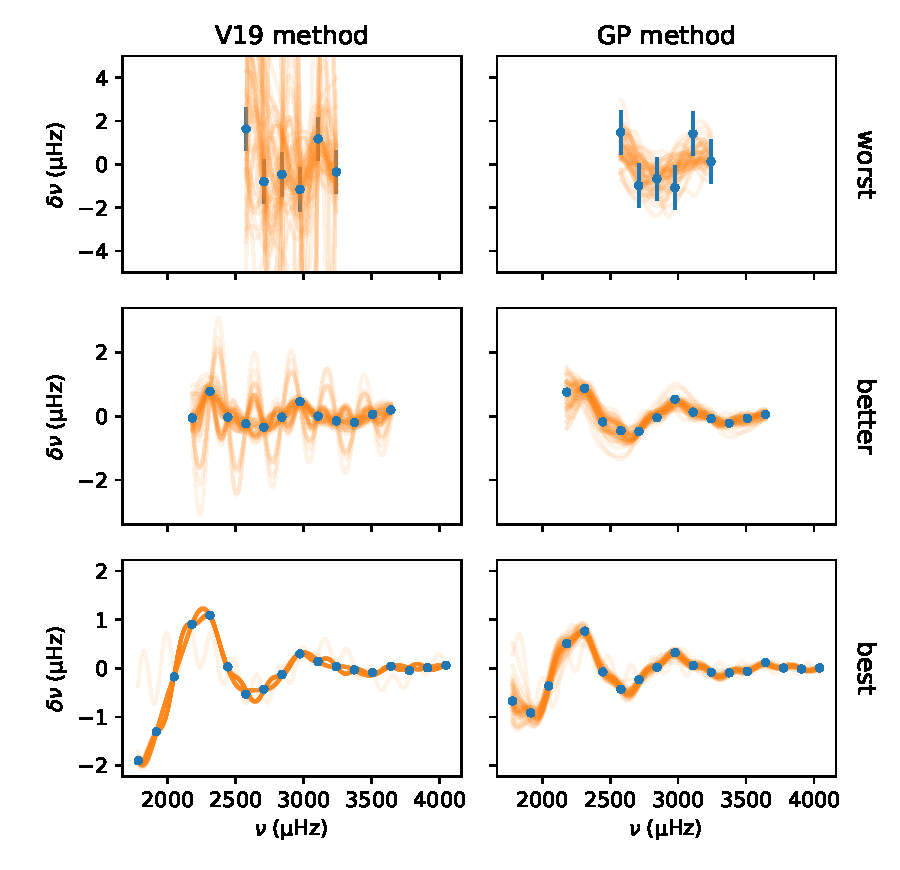
\includegraphics{figures/glitch-test-signal.pdf}
    \caption{50 random draws from the V19 and GP methods showing the total glitch signal, \(\delta\nu = \delta_\helium(\nu) + \delta_\bcz(\nu)\), as a function of frequency, \(\nu\). The data points plot in blue are the median smooth component model at \(\vect{n}\) subtracted from the observed modes \(\vect{\nu}_\obs\) with their observed uncertainty \(\sigma_\obs\).}
    \label{fig:glitch-test-signal}
\end{figure}

In Figure \ref{fig:glitch-test-signal}, we plot the predicted glitch signal, \(\delta\nu\), using 50 draws from the posterior distribution on the model parameters for both methods. We subtracted the median background component from the observed \(\nu_n\) over-plot. For each scenario, both methods predicted similar glitches. The \citetalias{Verma.Raodeo.ea2019} method has more extreme multimodality in all cases. For example, the better case showed a high-amplitude BCZ glitch solution which is not present with the GP method. This was likely because the GP method used a prior which reduced the probability of extreme solutions --- a consequence of the Bayesian methodology. The \citetalias{Verma.Raodeo.ea2019} method also appeared to be over-confident in its glitch solutions for the best case compared to the GP method. This is a sign that there was uncertainty in the \citetalias{Verma.Raodeo.ea2019} model not being accounted for. In the best-case scenario, the two methods appeared to differ at low frequency. We expect this is due to the different smooth background component.

\begin{figure}
    \centering
    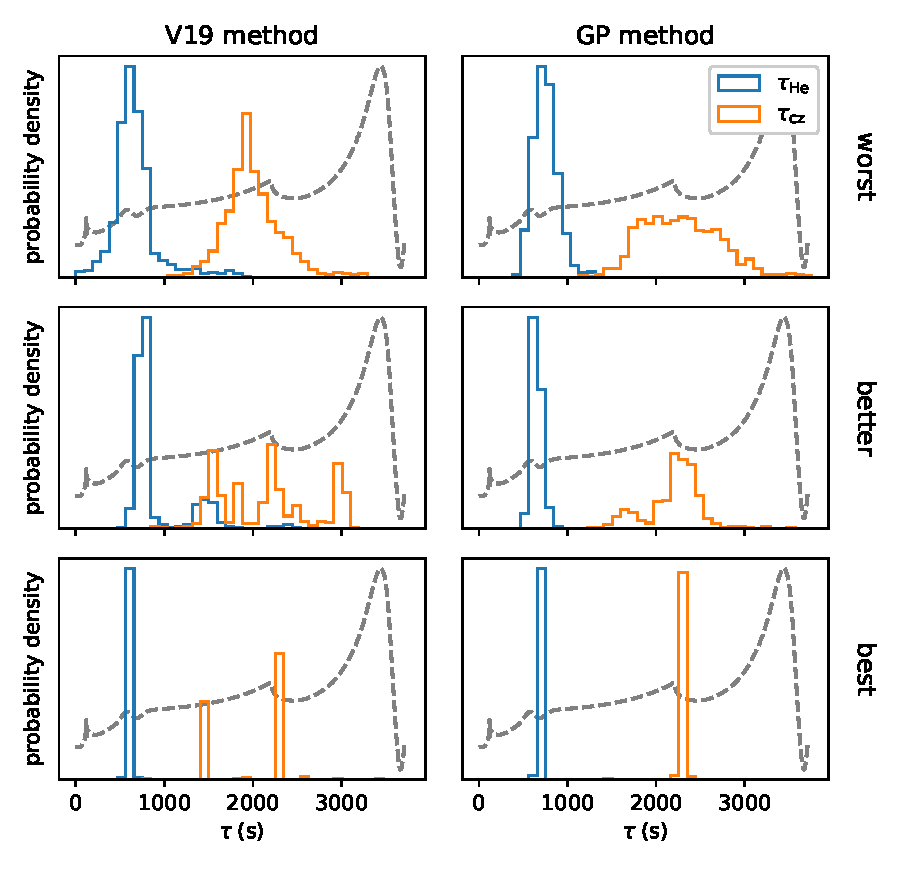
\includegraphics{figures/glitch-test-tau.pdf}
    \caption{Samples from the V19 and GP methods for the acoustic depths of the helium glitch (\(\tau_\helium\)) and base of the convective zone (\(\tau_\bcz\)). The sound-speed gradient from Figure \ref{fig:sound-speed-gradient} is over-plot with a grey dashed line.}
    \label{fig:glitch-test-tau}
\end{figure}

It was difficult to determine which method did a better job at finding glitch parameters. The glitch model is an approximation and the exact physical meaning of the parameters is unknown. However, we plotted posterior distributions of the glitch acoustic depths, \(\tau_\helium\) and \(\tau_\bcz\), in Figure \ref{fig:glitch-test-tau} and compared them to the sound speed gradient of the test star from Figure \ref{fig:sound-speed-gradient}. For the worst case, both methods gave broad distributions for the acoustic depths, compatible with their respective initial guesses and priors. The \citetalias{Verma.Raodeo.ea2019} method initial guesses appeared to underestimate \(\tau_\bcz\), whereas the GP method prior was broad enough to encompass a wide range of possible \(\tau_\bcz\). In the better and best cases, we found that the \citetalias{Verma.Raodeo.ea2019} had strong multimodality as a consequence of not incorporating an informed prior in their model. For example, the better case found solutions for \(\tau_\helium\) far deeper into the star than we would expect, at around \SI{1500}{\second} and \SI{2500}{\second}.

One problem with our choice of glitch functions, predicted by \citet{Houdek.Gough2007} and shown in \citet{Verma.Faria.ea2014}, is that the values for \(\tau_\helium\) obtained are under-predicted compared to the true location of the second ionisation of helium. This is because \(\delta_\helium(\nu)\) does not include the smaller glitch component due to the first ionisation of helium. This is located at a slightly lower \(\tau\), so the period of the resulting glitch fit is slightly increased. We can see this for the fit to the best star with the \citetalias{Verma.Raodeo.ea2019} method in Figure \ref{fig:glitch-test-tau}. The respective solutions for \(\tau_\helium\) from the GP method are more compatible with the location of the second ionisation trough \todo{quantify this}. This could be a result of the GP doing a better job of absorbing the first helium ionisation component than the 4-th order polynomial.

\todo{include numbers for \(\tau\) in a table compared with \(\tau\) from the }

\begin{figure}
    \centering
    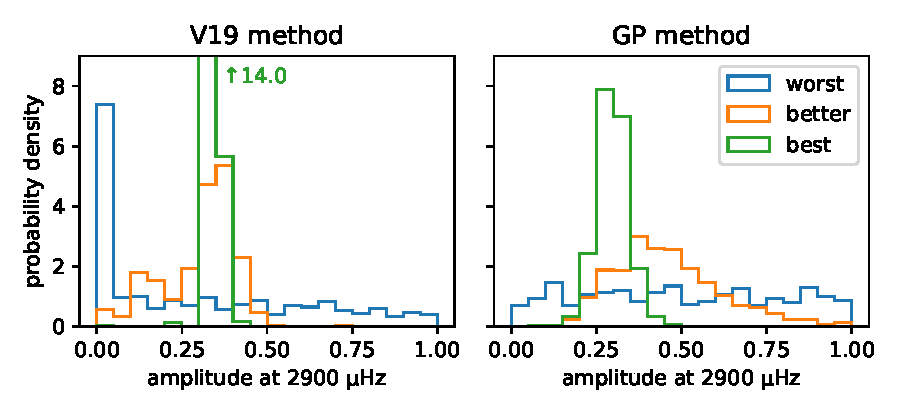
\includegraphics{figures/glitch-test-amplitude.pdf}
    \caption{Samples of the helium glitch amplitude at a reference frequency of \SI{3000}{\micro\hertz} fit with the V19 and GP methods for the worst-, better-, and best-case test data. The tallest bar in the V19 method panel is cropped with its value displayed in green text.}
    \label{fig:glitch-test-amplitude}
\end{figure}

Using the glitch parameters as a helium diagnostic could involve measuring the amplitude of the helium glitch at a reference frequency such as \(\nu_{\max}\). We should expect solutions for this reference amplitude (\(A_\mathrm{ref}\)) to converge on a value as the data quality increases from worst to best. It is also important that the uncertainty of the reference amplitude is accurate if using it to constrain helium abundance in a population of stars. We compared reference amplitudes at \(\nu_\mathrm{ref}\) from both methods in Figure \ref{fig:glitch-test-amplitude}. The \citetalias{Verma.Raodeo.ea2019} method preferred low-amplitude solutions for the worst and better cases than the best case. If using this method on a population of stars, this could bias inference towards lower values of helium abundance. On the other hand, the GP method reflects our prior in the worst case, with the width of the distribution shrinking as the data improves. In the best case, the \citetalias{Verma.Raodeo.ea2019} method found \(A_\helium^\mathrm{ref} = 0.347_{-0.005}^{+0.006}\), whereas the GP method found \(A_\helium^\mathrm{ref} = 0.296_{-0.036}^{+0.042}\).

In both methods, the samples for \(\alpha_\helium\) and \(\beta_\helium\) were correlated. This was expected, because larger values of \(\beta_\helium\) can be compensated for with a larger amplitude factor \(\alpha_\helium\). In the GP method, we did not include this expected correlation in our prior. However, in future work, we should devise a multivariate prior for the amplitude parameters to account for this. We found that having broader priors on \(\alpha_\helium\) and \(\beta_\helium\) lead to the model predicting unrealistic glitches. Our ability to test the influence of the prior is limited if we cannot relax its effect.

A potential limitation of the GP method is that we calculate the glitch at \(\tilde{\nu}_n\) from the linear asymptotic equation (Equation \ref{}). In regions where the gradient of \(\delta(\nu)\) and the difference between \(\tilde{\nu}_n\) and the true frequency are high, this leads to notable differences between the mean function and the true frequency (\(\sim \SI{0.1}{\micro\hertz}\)) which the GP kernel function cannot absorb. We accounted for this uncertainty due to this by adding Gaussian noise parametrised by \(\sigma\). However, for the best star, \(\sigma \approx 0.05\) which is larger than the observational uncertainty \(\sigma_\obs = 0.01\). This limits our method's inference ability for the best asteroseismic targets. One solution is to replace \(\tilde{\nu}_n\) with a quadratic \citep[e.g.][]{Nielsen.Davies.ea2021} which better approximates \(\nu_n\). Alternatively, we could use Newton's method to solve the mean function for \(\nu\).

% \todo{Why not use delta gamma / gamma as the probe of helium abundance? That is proportional to alpha / sqrt(beta). Then, an update to this method can use this and beta as a parameter and then work out alpha from that, since beta should scale with tau and the depth is a signature of helium abundance. Be careful as number of modes correlates with delta nu value of fit.}

% \todo{Comment on how V19 stuggles to find DY/DZ with their method, and finds unusually low values of initial helium. This could be a result of their fitting method.}

\subsubsection{16 Cyg A}

Figure \ref{fig:glitch-16cyga} compares the results from both methods applied to the 16 Cyg A data. We found that the \citetalias{Verma.Raodeo.ea2019} method predicted extreme solutions for the glitch where the GP method did not. This was compatible with our findings in the previous section, and likely arose due to the use of a prior in the GP method. There was also a difference of about \SI{0.5}{\micro\hertz} at the low frequencies such that the \citetalias{Verma.Raodeo.ea2019} predicted a larger glitch amplitude. Again, this was seen in the previous section, particularly for the best-case scenario. This was caused by the difference in smooth background models, with the GP appearing to be more flexible than the polynomial. In future work, we could test the accuracy of the GP background by making predictions for lower \(n\) modes and seeing which method does better. Otherwise, the two methods gave similar predictions for the glitch function. 

The \citetalias{Verma.Raodeo.ea2019} method found \(\tau_\helium = 917_{-53}^{+50} \, \mathrm{s}\) and our GP method obtained \(\tau_\helium = 931_{-88}^{+59} \, \mathrm{s}\), within 1-\(\sigma\) of each other. The large lower uncertainty from the GP method result could arise from our method picking up the small signal due to He\,\textsc{i} ionisation. As found in the previous section, our method finds a slightly larger value of \(\tau_\helium\) than the \citetalias{Verma.Raodeo.ea2019} method, although not significantly in this case. Both methods found \(\tau_\helium\) to within 1-\(\sigma\) of the result of \SI{930(14)}{\second} when fit to \(l=0,1,2\) modes in \citet{Verma.Faria.ea2014}.

For both methods, we calculated the helium glitch amplitude at a reference frequency of \SI{2188.5}{\micro\hertz} equivalent to the value of \(\nu_{\max}\) obtained by \citet{Lund.SilvaAguirre.ea2017}. Samples from their posteriors are shown in the bottom panel of Figure \ref{fig:glitch-16cyga}. We found \(A_\helium^\mathrm{ref} = 0.260_{-0.065}^{+0.050}\) for the \citetalias{Verma.Raodeo.ea2019} method, and \(A_\helium^\mathrm{ref} = 0.333_{-0.073}^{+0.081}\) for the GP method. Both values were about 1-\(\sigma\) apart.

\begin{figure}
    \centering
    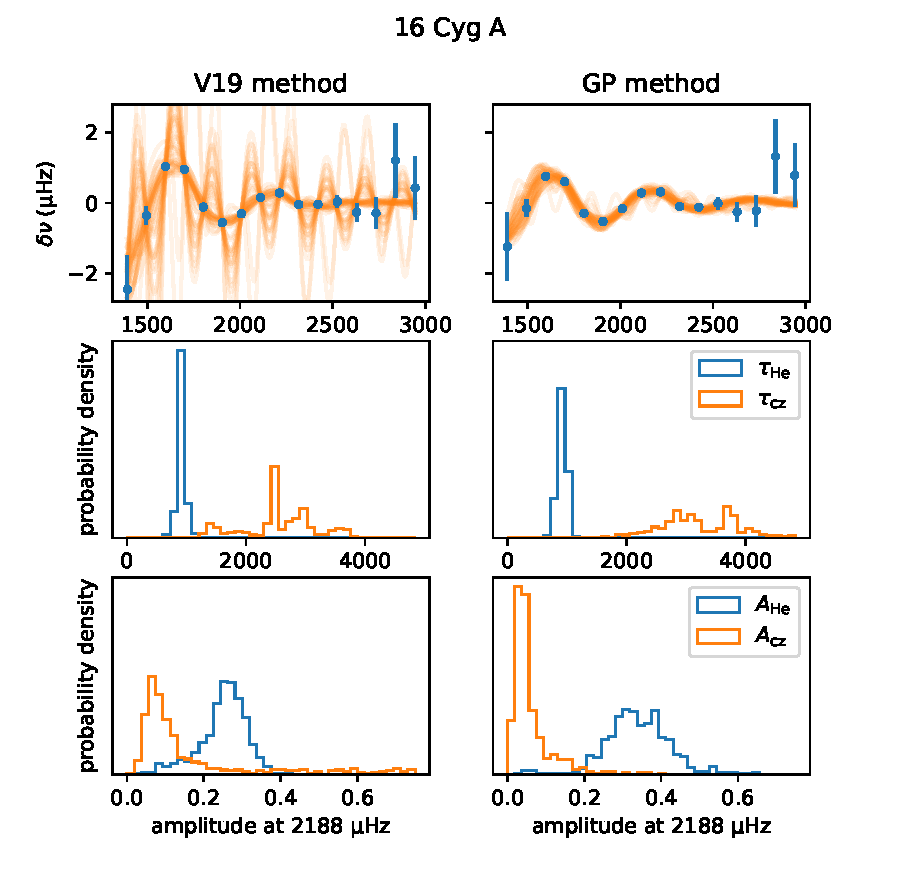
\includegraphics{figures/glitch-16cyga.pdf}
    \caption{Results for the glitch fit to 16 Cyg A using the \citetalias{Verma.Raodeo.ea2019} method (\emph{left}) and GP method (\emph{right}). The top panel shows 50 draws from the posterior prediction of \(\delta\nu = \delta_\helium(\nu) + \delta_\bcz(\nu)\) with the observed \(\nu_n\) minus the median smooth background component of the model. The middle and bottom panels shows the posterior sample probability density for the acoustic depths and reference amplitudes of the glitches respectively.}
    \label{fig:glitch-16cyga}
\end{figure}

\subsubsection{Improvements to the model}

It is important that the GP model has a robust and physically motivated prior. However, some assumptions we have made could lead to an incorrect prior and bias the results. For example, the outer convective zone gets shallower for hotter stars (approaching \(\teff \approx \SI{7000}{\kelvin}\)) making the assumption that \(\tau_\bcz/\tau_0 \approx 0.6\) an overestimate. There is a notable temperature dependence to \(\tau_\bcz/\tau_0\) observed in the grid of stellar models which could instead be exploited when constructing the prior. Additionally, there is strong correlation between the helium amplitude parameters \(\alpha_\helium\) and \(\beta_\helium\). For our prior to reflect realistic glitches, these parameters should be drawn from a multivariate distribution parametrised by their covariance.

% \todo{In discussion can show some plots of \(\tau/\tau_0\) in model stars and how they relate to temperature, could use temperature to influence prior.}

Once the GP method is good enough to run on the grid of stellar models, we could use the results to inform an empirical prior to then apply to observed stars. This could lead to some model-dependence but the prior could be relaxed slightly to account for this.

\todo{Conclusion}
